\documentclass[11pt,a4paper]{article}
\usepackage[T1]{fontenc}
\usepackage[utf8]{inputenc}
\usepackage{lmodern}
\usepackage[margin=28mm]{geometry}
\usepackage{amsmath,amssymb,amsthm,mathtools,mathrsfs}
\usepackage{microtype}
\usepackage{booktabs,array}
\usepackage{tikz}
\usetikzlibrary{arrows.meta,positioning}
\usepackage{xcolor}
\usepackage[nottoc,notlof,notlot]{tocbibind}
\usepackage{needspace}
\usepackage[colorlinks=true,linkcolor=blue!45!black,citecolor=blue!45!black,urlcolor=blue!45!black,bookmarksdepth=2]{hyperref}
\hypersetup{pdftitle={Stabilizer orbits and thick tensor ideals of dualizable K(n)-local spectra},pdfauthor={OpenAI}}
\setcounter{tocdepth}{1}
\numberwithin{equation}{section}
\newtheorem{theorem}{Theorem}[section]
\newtheorem{proposition}[theorem]{Proposition}
\newtheorem{lemma}[theorem]{Lemma}
\newtheorem{corollary}[theorem]{Corollary}
\newtheorem{conjecture}[theorem]{Conjecture}
\theoremstyle{definition}
\newtheorem{definition}[theorem]{Definition}
\theoremstyle{remark}
\newtheorem{remark}[theorem]{Remark}
\newcommand{\Qp}{\mathbb Q_p}
\newcommand{\Zp}{\mathbb Z_p}
\newcommand{\Fp}{\mathbb F_p}
\newcommand{\Cp}{\mathbb C_p}
\newcommand{\OO}{\mathcal O}
\newcommand{\mm}{\mathfrak m}
\DeclareMathOperator{\End}{End}
\DeclareMathOperator{\Hom}{Hom}
\DeclareMathOperator{\Lie}{Lie}
\DeclareMathOperator{\Spec}{Spec}
\DeclareMathOperator{\Spf}{Spf}
\DeclareMathOperator{\Spc}{Spc}
\DeclareMathOperator{\Perf}{Perf}
\DeclareMathOperator{\Supp}{Supp}
\DeclareMathOperator{\Ann}{Ann}
\DeclareMathOperator{\rank}{rank}
\DeclareMathOperator{\height}{ht}
\DeclareMathOperator{\im}{im}
\DeclareMathOperator{\id}{id}
\DeclareMathOperator{\GL}{GL}
\DeclareMathOperator{\Frac}{Frac}
\title{Stabilizer orbits and thick tensor ideals\\of dualizable \(K(n)\)-local spectra}
\author{OpenAI}
\date{September 24, 2026}
\begin{document}
\maketitle
\begin{abstract}
We classify the prime and radical ideals of the Lubin--Tate deformation
ring invariant under an open Morava stabilizer subgroup, at every prime
and positive height.  This proves Chai's invariant-ideal conjecture in
the standard finite-residue-field formulation.  It also proves the
Hovey--Strickland conjecture: the dualizable \(K(n)\)-local category has
exactly \(n+2\) thick tensor ideals, and its Balmer spectrum is a chain
of \(n+1\) points.
\end{abstract}
\tableofcontents
\section{Introduction}\label{sec:introduction}

Chromatic height organizes both the deformation theory of formal groups
and the tensor structure of stable homotopy theory.  Two classification
problems ask whether height accounts for all the relevant closed
subobjects: the invariant ideals in a Lubin--Tate deformation ring, and
the thick tensor ideals of dualizable Morava-local spectra.  We prove
both classifications, using the arithmetic problem as the main step.

Fix a prime \(p\) and an integer \(n\geq1\).  Let \(\Gamma_n\) be the
height-\(n\) Honda formal group, let \(A_n\) be its endomorphism ring over
\(\overline{\mathbb F}_p\), and put
\[
 E_0=W(\mathbb F_{p^n})[[u_1,\ldots,u_{n-1}]],
 \qquad I_0=0,\qquad
 I_h=(p,u_1,\ldots,u_{h-1})\quad(1\leq h\leq n).
\]
The ring \(E_0\) represents its marked deformations.  The ideals \(I_h\)
are the height ideals: in characteristic \(p\), their vanishing specifies
where the formal group has height at least \(h\).
The nonextended Morava stabilizer \(A_n^\times\) acts by changing the
marking.  The canonical extended stabilizer \(G_n\) also includes the
residue-field Galois action.  The unit ideal is listed separately from
the proper ideals.

\begin{theorem}[Stabilizer-invariant ideals]\label{thm:invariant-radicals}
Let \(U\subseteq A_n^\times\) be any open subgroup.
The proper prime ideals of \(E_0\) stabilized by \(U\) are precisely
\[
 0,\ I_1,\ldots,I_n.
\]
The \(U\)-invariant radical ideals are precisely
\[
 0,\ I_1,\ldots,I_n,\ E_0.
\]
The latter list also gives the radical ideals invariant under the full
canonical \(G_n\)-action.
\end{theorem}

This proves the invariant-ideal assertion called Chai's Hope in the
finite-residue-field formulation of
\cite[Hope~4.1 and Remark~4.2]{BHN22}, and extends that formulation
from the full stabilizer to every open subgroup.  The open-subgroup
scope also occurs in Chai's original closed-fiber question, as explained
in \cite[Remark~4.2]{BHN22}.  The second classification concerns Honda
Morava \(E\)-theory \(E\) with coefficient ring \(E_0\), and the
homotopy category \(\mathcal D_{(n,p)}\) of dualizable \(K(n)\)-local
spectra.  Its tensor product and unit are
\[
 X\otimes Y=L_{K(n)}(X\wedge Y),
 \qquad \mathbf 1=L_{K(n)}S.
\]
A thick tensor ideal is a full subcategory closed under equivalences,
finite sums, suspensions and desuspensions, cofiber sequences, retracts,
and tensoring with every object of \(\mathcal D_{(n,p)}\).
Dualizability is essential here: it is more general than compactness in
the \(K(n)\)-local category \cite[Theorems~8.5--8.6]{HS99}.

A finite \(p\)-local spectrum \(F\) has \emph{type \(k\)} if
\(K(i)_*F=0\) for \(i<k\) and \(K(k)_*F\neq0\), with
\(K(0)=H\mathbb Q\).  Such spectra exist in every type: start with the
sphere and the degree-\(p\) cofiber, and then take cofibers of the
self-maps supplied by the Hopkins--Smith periodicity theorem
\cite[Definition~8 and Theorem~9]{HopkinsSmith98}.
For \(0\leq k\leq n\), choose a finite type-\(k\) spectrum \(F(k)\)
and put
\[
 \mathcal D_k=\big\langle L_{K(n)}F(k)\big\rangle_\otimes,
 \qquad \mathcal D_{n+1}=0,
\]
where the brackets mean the generated thick tensor ideal in
\(\mathcal D_{(n,p)}\).

\begin{theorem}[Hovey--Strickland conjecture]\label{thm:main}
For every prime \(p\) and every \(n\geq 1\), the thick tensor ideals of
\(\mathcal D_{(n,p)}\) are exactly
\[
 \mathcal D_{(n,p)}=\mathcal D_0
 \supsetneq\mathcal D_1\supsetneq\cdots
 \supsetneq\mathcal D_n\supsetneq\mathcal D_{n+1}=0.
\]
In particular, there are \(n+2\) such ideals, and each \(\mathcal D_k\)
is independent of the chosen finite type-\(k\) spectrum.
\end{theorem}

The Balmer spectrum of a tensor category is the space of its prime thick
tensor ideals.  Corollary~\ref{fin:balmer} identifies this spectrum here
with the \(n+1\) proper members of the displayed chain, including the
zero ideal.  It also specifies their specialization order and the
support of each finite type generator.

\subsection{History and the two classification problems}

The thick subcategory theorem of Hopkins and Smith classifies thick
subcategories of finite spectra by chromatic type, while their
periodicity theorem supplies the corresponding self-maps
\cite[Theorems~7 and~9]{HopkinsSmith98}.  Hovey and Strickland proposed
the dualizable \(K(n)\)-local counterpart in their study of Morava
\(K\)-theory and localization \cite[Section~12, p.~61]{HS99}.
Their Problem~16.8 also asks directly about stabilizer-invariant primes
and radical ideals of the deformation ring; it explains why the
invariant-prime theorem for ordinary complex cobordism does not by
itself answer this question.

Chai studied the action on the closed fiber of Lubin--Tate space and
proposed that invariant irreducible formal loci should be height loci
\cite{Chai96}.  We use the precise formulation and comparison of
coefficient fields and group actions in
\cite[Section~4, Hope~4.1 and Remark~4.2]{BHN22}.
Formal rigidity also has an established role in Chai's work on
\(p\)-divisible formal groups \cite{Chai08}.  The formal-closure
argument below belongs to this general circle of ideas, but starts
from a subgroup of Honda-group points and proves its required
annihilator statement directly.

Barthel, Heard, and Naumann proved the Hovey--Strickland conjecture at
height two for every prime and established the general implication from
Chai's invariant-ideal assertion to the spectral classification
\cite[Theorems~4.9 and~4.15]{BHN22}.  The descent and support methods in
that implication build on Mathew's work on Morava \(E\)-theory descent
\cite{Mathew16} and Balmer's tensor-nilpotence criterion for surjectivity
on spectra \cite{Balmer18}.  We recall the exact support comparison in
Proposition~\ref{fin:support}.  Its direction is unrestricted in \(p\).
The inequality \(2p-2>n^2+n\) in \cite[Theorem~4.13]{BHN22}
concerns the converse, which uses realization of Morava modules.

The generic-fiber part has earlier Lie-theoretic precedents.
Barthel--Heard--Naumann credit Chai with an unpublished
characteristic-zero invariant-ideal result and use the Gross--Hopkins period map to study
projective stabilizer orbits
\cite[Remark~4.2 and Proposition~4.18]{BHN22}.
We retain a local analytic-germ proof of the needed conclusion.
The main issue addressed here is the characteristic-\(p\) height
strata, where infinitesimal stabilizer directions alone do not give
the required control of invariant equations.

Recent generation and comparison results concern related categories.
Lee and Pstr{\k a}gowski identify the category of locally fp spectra,
which contains the dualizable \(K(n)\)-local spectra as well as
nondualizable objects
\cite[Example~1.6 and Theorems~1.7--1.9]{LP26}.
Surjectivity of the map from the \(K(n)\)-local to the \(E(n)\)-local
Balmer spectrum was established by Barthel--Heard--Naumann
\cite[Remark~3.6]{BHN22}; Balmer--Sanders give a later general treatment
\cite[Proposition~8.11 and Remark~8.13]{BalmerSanders}.
These results provide generation and surjectivity statements.
The arithmetic theorem above classifies the invariant supports needed
to determine the entire ideal lattice.

\begin{figure}[htbp]
\centering
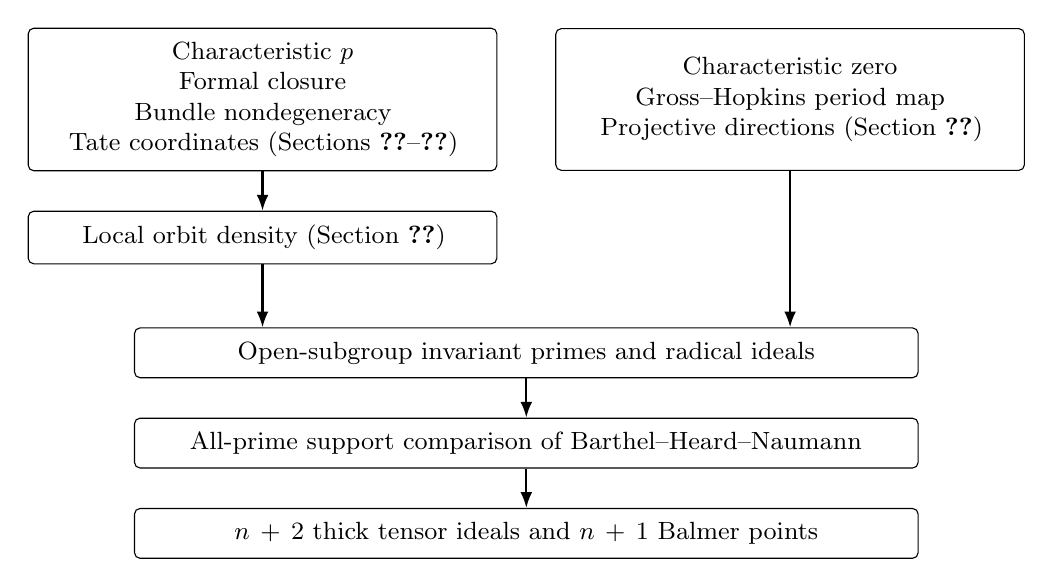
\begin{tikzpicture}[
  box/.style={draw,rounded corners=2pt,align=center,font=\small,
              inner sep=5pt,text width=5.6cm},
  merge/.style={box,text width=9.6cm},
  flow/.style={-{Latex[length=2mm]},thick}
]
\node[box,minimum height=1.8cm] (charp) at (-3.35,0)
  {Characteristic $p$\\Formal closure\\Bundle nondegeneracy\\
   Tate coordinates (Sections~\ref{sec:formal}--\ref{sec:deformations})};
\node[box,minimum height=1.8cm] (charzero) at (3.35,0)
  {Characteristic zero\\Gross--Hopkins period map\\
   Projective directions (Section~\ref{sec:classification})};
\node[box,below=5mm of charp] (density)
  {Local orbit density (Section~\ref{sec:orbits})};
\node[merge,below=8mm of density.south,xshift=3.35cm] (primes)
  {Open-subgroup invariant primes and radical ideals};
\node[merge,below=5mm of primes] (support)
  {All-prime support comparison of Barthel--Heard--Naumann};
\node[merge,below=5mm of support] (spectra)
  {$n+2$ thick tensor ideals and $n+1$ Balmer points};
\draw[flow] (charp) -- (density);
\draw[flow] (density.south) -- (density.south |- primes.north);
\draw[flow] (charzero.south) -- (charzero.south |- primes.north);
\draw[flow] (primes) -- (support);
\draw[flow] (support) -- (spectra);
\end{tikzpicture}

\caption{The two orbit arguments classify invariant primes.  Only the
characteristic-\(p\) branch uses the formal, bundle, and deformation
constructions of Sections~\ref{sec:formal}--\ref{sec:deformations}.
The arithmetic branches join before the all-prime support comparison.}
\label{fig:proof-flow}
\end{figure}

\subsection{The argument}

Set \(C=\Cp^\flat\) and \(k=\overline{\mathbb F}_p\), viewed as the
coefficient field in \(C\), and write
\(\mm_C=\{c\in C:|c|<1\}\).  Fix a characteristic-\(p\) point \(x\)
of formal height \(1\leq h<n\).  The main task is to show that a
nonzero analytic germ at \(x\) on the height-at-least-\(h\) parameter locus
\(I_h=0\) cannot vanish on the stabilizer orbit of \(x\).
The finite kernels of the universal deformation give a height-\(n\)
algebraic \(p\)-divisible group.  At \(x\), its connected part has
height \(h\) and its \'{e}tale quotient has height \(r=n-h\).
The universal-cover comparison lets us regard a basis
\(z_1,\ldots,z_r\) of its \'{e}tale Tate module as points of the
perfected height-\(n\) Honda group.  Specializing these fixed vectors
at nearby parameters in this locus gives analytic functions \(\theta_i\) vanishing
at \(x\).  Their vanishing tests whether the vectors remain in the
nearby Tate lattice.  Section~\ref{sec:deformations} proves that their
parameter differential is invertible: a vector in its kernel splits
the \'{e}tale quotient over the dual numbers, fixed-height rigidity
makes the connected factor constant, and the Kodaira--Spencer map
then kills the parameter vector
(Proposition~\ref{def:coordinates}).

Put \(q=p^h\).  For a fixed \(d\in A_n\), let
\(y_N=(1-p^Nd)\cdot x\); these points tend to \(x\).
Stabilizer transport relates \(\theta_i(y_N)\) to multiplication by
\(p^N\) in the formal group at \(y_N\).  Integral comparison series
intertwining multiplication by \(p\) with that of the height-\(h\)
Honda group turn this relation into coordinatewise Frobenius powers.
Applying these series to the specializations of \(z_i\) and
\(dz_i\) at \(y_N\) gives tuples \(U_N\) and \(s_N\), respectively,
in \(\mm_C^r\).  Theorem~\ref{orb:density} proves the exact identity
and limit
\[
 U_N=s_N^{q^N},\qquad
 s_N\longrightarrow s(d)=\bigl(\nu_x(dz_1),\ldots,\nu_x(dz_r)\bigr),
\]
where \(\nu_x\) is specialization at \(x\) followed by an integral
formal identification with the height-\(h\) Honda group.
Proposition~\ref{def:natural-comparison} makes \(\nu_x\) a nonzero
natural map on perfectoid test spaces.  The corresponding change of
parameter coordinates is formal.  To compare it with the numerical
tuples \(U_N\), we match any fixed finite number of analytic
coefficient germs and bound the remaining integral tails
(Lemma~\ref{orb:finite-jets}).  The coefficient germs may have
shrinking domains; the estimates require only one finite jet at a time.

Suppose a nonzero analytic germ \(P\) vanishes on the orbit.  Its expansion
in the formal coordinates has fixed coefficients \(B_\ell\), chosen
before \(d\).  Finite truncation followed by \(q^N\)-th roots gives
bounds on the finite sums
\(\sum_{|\ell|\leq m} B_\ell^{1/q^N}s(d)^\ell\).
Frobenius separation (Lemma~\ref{formal:separation}) turns these
bounds into a single nonzero formal equation over \(k\) on the subgroup
\[
 S_x=\{\bigl(\nu_x(dz_1),\ldots,\nu_x(dz_r)\bigr):d\in A_n\}.
\]
The formal-closure argument in Section~\ref{sec:formal} then produces
a nonzero row of Honda endomorphisms annihilating \(S_x\)
(Proposition~\ref{formal:closure}).

The contradiction is geometric.  The Fargues--Fontaine curve
\cite{FF18} and Le Bras's theorem on Banach--Colmez sheaves
\cite{LeBras18} turn this natural endomorphism relation into a
vector-bundle relation.  A degree-one determinant argument promotes
the \(\Qp\)-independence of \(z_1,\ldots,z_r\) to independence at the
generic point of the curve (Lemma~\ref{bundles:independence}).
There the division algebra action spans the full matrix algebra.
A matrix selecting one of these independent vectors contradicts the
nonzero endomorphism row
(Proposition~\ref{bundles:nondegeneracy}).  Thus \(P\) must be zero.
This vanishing property is the \emph{local orbit density} proved in
Theorem~\ref{orb:density}.

Section~\ref{sec:classification} uses this result to classify invariant
primes containing \(p\).  Primes in characteristic zero are handled
separately by the Gross--Hopkins period map \cite{GH94,HG94Bundles}.
A finite minimal-prime argument classifies invariant radical ideals,
and the established support comparison transfers the height chain to
thick tensor ideals and their Balmer spectrum.  The final description
also identifies the support map from \(\Spec(E_0)\): each height stratum
maps to one Balmer point.  Figure~\ref{fig:proof-flow} records the two
arithmetic branches and where they enter the spectral argument.

\section{Frobenius separation and formal closure}\label{sec:formal}

We first establish a rigidity statement for subgroups of products of a Honda
formal group. A formal equation over the residue field will force such a
subgroup to satisfy a nonzero homomorphism equation. The first step separates
coefficients by taking increasingly deep Frobenius roots.

\subsection{Fields and Honda formal groups}

Fix a prime $p$. Throughout the proof, put
\[
  k=\overline{\Fp},\qquad C=\Cp^{\flat},
\]
and fix the coefficient-field embedding $k\hookrightarrow\OO_C$ inducing
the identification of the residue field with $k$. The field $C$ is
algebraically closed, complete, and of characteristic $p$. We write
$\mm_C=\{c\in C:|c|<1\}$ and use the maximum norm on finite tuples.
Every nonzero element of $k$ has norm one. Consequently a formal power
series over $k$ can be evaluated at any tuple in $\mm_C^r$.

For $s\geq 1$, set $q_s=p^s$ and $k_s=\mathbb F_{q_s}$. The Lubin--Tate formal-module construction for the unramified extension
of $\Qp$ of degree $s$, applied to the series $pT+T^{q_s}$
\cite[Theorem~1]{LT65}, gives on reduction a one-dimensional
commutative Honda formal group $\Gamma_s$ over $k_s$ with
\[
  [p]_{\Gamma_s}(T)=T^{q_s}.
\]
Write
\[
  A_s=\End_k(\Gamma_s),\qquad \Delta_s=A_s[1/p].
\]
The classification of one-dimensional formal groups
\cite[Theorem~18.5.1]{Hazewinkel78} identifies every formal group of
height $s$ over an algebraically closed field of characteristic $p$
with $\Gamma_s$. Dieudonn\'e theory over perfect fields
\cite[Chapter~III, \S8; Chapter~IV, \S\S1,3--4]{Demazure72}
shows that its associated $p$-divisible group is simple up to isogeny
and that $\Delta_s$ is a central division algebra over $\Qp$ of
dimension $s^2$. The isogeny category of $p$-divisible groups over $k$
is semisimple.
These statements include height one and the prime two.

Every endomorphism of $\Gamma_s$ is defined over $k_s$. Indeed, if
$a(T)=\sum_{j\geq1}a_jT^j$ is such an endomorphism, its commutation
with multiplication by $p$ gives
\[
  a(T^{q_s})=a(T)^{q_s},
\]
so $a_j^{q_s}=a_j$ for all $j$. We use formal-group addition in
$\Gamma_s$ and its products; ordinary sums of power-series coefficients
and ordinary differences of coordinates retain their usual meaning.

\subsection{Separating coefficients}

For a multi-index $\ell=(\ell_1,\ldots,\ell_r)\in\mathbb N^r$, put
$|\ell|=\sum_i\ell_i$ and $T^\ell=\prod_i T_i^{\ell_i}$. Roots under
Frobenius in $C$ are unique.
For a related separation argument using high Frobenius substitutions,
see \cite[Proposition~3.1]{Chai08}.

\begin{lemma}[Frobenius separation]\label{formal:separation}
Let $h,r\geq1$, put $q=p^h$, and let $(b_\ell)_{\ell\in\mathbb N^r}$
be an arbitrary family in $C$. Suppose $s\in\mm_C^r$ satisfies, for
every integer $m\geq0$,
\begin{equation}\label{formal:root-bound}
  \limsup_{N\longrightarrow\infty}
  \left|\sum_{|\ell|\leq m} b_\ell^{1/q^N}s^\ell\right|
  \leq \|s\|^{m+1}.
\end{equation}
Then, for every $k$-linear functional $\lambda:C\to k$,
\[
  \sum_{\ell\in\mathbb N^r}\lambda(b_\ell)s^\ell=0.
\]
The series in this conclusion converges, and no continuity assumption
on $\lambda$ is required.
\end{lemma}

\begin{proof}
Fix $m$. If all the coefficients through degree $m$ vanish, the
corresponding assertion is immediate. Otherwise choose a $k$-basis
$\beta_1,\ldots,\beta_a$ for their span and write
\[
  b_\ell=\sum_{j=1}^a c_{\ell j}\beta_j,
  \qquad c_{\ell j}\in k\quad (|\ell|\leq m).
\]
There is a subsequence of positive integers $N$ on which $q^N$-power
Frobenius fixes all the $c_{\ell j}$: finitely many elements of
$\overline{\Fp}$ lie in a common finite field. On this subsequence,
\[
  \sum_{|\ell|\leq m}b_\ell^{1/q^N}s^\ell
  =\sum_{j=1}^a\beta_j^{1/q^N}v_j,
  \qquad v_j=\sum_{|\ell|\leq m}c_{\ell j}s^\ell.
\]
Put $V=\max_j|v_j|$. If $V>0$, choose $j_0$ with $|v_{j_0}|=V$,
set $w_j=v_j/v_{j_0}$, and let $\rho_j\in k$ be the residue of
$w_j\in\OO_C$. At least one $\rho_j$ is nonzero, and
\[
  \eta:=\max_j|w_j-\rho_j|<1.
\]
Pass to a further subsequence on which $q^N$-power Frobenius also fixes
all the $\rho_j$. The independence of the $\beta_j$ gives
$\sum_j\beta_j\rho_j\ne0$, whence
\[
  \left|\sum_j\beta_j^{1/q^N}\rho_j\right|
  =\left|\sum_j\beta_j\rho_j\right|^{1/q^N}
  \longrightarrow1.
\]
On the other hand,
\[
  \limsup_N
  \left|\sum_j\beta_j^{1/q^N}(w_j-\rho_j)\right|
  \leq\eta<1,
\]
since $|\beta_j|^{1/q^N}\to1$ for every $j$. The ultrametric
inequality therefore implies
\[
  \left|\sum_j\beta_j^{1/q^N}v_j\right|\longrightarrow V
\]
along this subsequence. Equation~\eqref{formal:root-bound} gives
$V\leq\|s\|^{m+1}$; this inequality also holds if $V=0$.

For an arbitrary $k$-linear functional $\lambda$, we now have the
finite-sum estimate
\[
  \left|\sum_{|\ell|\leq m}\lambda(b_\ell)s^\ell\right|
  =\left|\sum_j\lambda(\beta_j)v_j\right|
  \leq V\leq\|s\|^{m+1}.
\]
Here $|\lambda(\beta_j)|\leq1$, because these values lie in $k$.
The series with coefficients $\lambda(b_\ell)\in k$ converges at
$s$, and the last bound tends to zero as $m\to\infty$. At $s=0$,
Equation~\eqref{formal:root-bound} for $m=0$ forces $b_0=0$, giving
the same conclusion.
\end{proof}

\begin{remark}\label{formal:separation-quantifiers}
The family $b_\ell$ need not be bounded. All uses of $\lambda$ in
the proof concern finite sums. Moreover, the conclusion holds for
\emph{every} $\lambda$ at each tuple satisfying the hypothesis.
Thus, if the same family satisfies Equation~\eqref{formal:root-bound}
at every point of a set, one may choose a single $\lambda$ nonzero on
one prescribed nonzero $b_\ell$ and obtain a common nonzero formal
equation over $k$ on that set. The Frobenius subsequences used to prove
the estimates may depend on the tuple and on $m$.
\end{remark}

\subsection{Reduced formal subgroups}

To prove formal closure, we will show that the ideal of all equations
vanishing on a subgroup of points defines a reduced formal subgroup.
The next two lemmas turn that formal subgroup into a nonzero
homomorphism equation. We first prove smoothness, before its dimension
or irreducibility is known. The use of ordinary differentials is
justified by the finite Frobenius expansion over a perfect coefficient
field.

\begin{lemma}\label{formal:reduced-smooth}
Let $\mathcal G$ be a smooth formal group over $k$ of dimension $r$,
with coordinate ring $R=k[[T_1,\ldots,T_r]]$. If
$\mathcal H\subseteq\mathcal G$ is a reduced closed formal subgroup,
then $\mathcal H$ is smooth. More precisely, for
$B=R/I$, with augmentation ideal $\mathfrak m_B$, put
$e=\dim_k(\mathfrak m_B/\mathfrak m_B^2)$. Then
$B\cong k[[X_1,\ldots,X_e]]$ as a complete local $k$-algebra.
\end{lemma}

\begin{proof}
Every $f\in R$ has a unique finite decomposition
\[
  f=\sum_{0\leq a_i<p}T_1^{a_1}\cdots T_r^{a_r}f_a(T)^p.
\]
An ordinary $k$-derivation kills all the $p$th powers, so this identity
shows that it is determined by its values on the $T_i$, through the
usual formal partial derivatives. Those partial derivatives themselves
are derivations. Hence the ordinary module $\Omega^1_{R/k}$ is free
on $dT_1,\ldots,dT_r$, and the quotient presentation gives
\begin{equation}\label{formal:differential-presentation}
  \Omega^1_{B/k}
  \cong B^r\big/
  \left\langle
    \bigl(\partial_1f,\ldots,\partial_rf\bigr):f\in I
  \right\rangle_B.
\end{equation}
In particular, this ordinary differential module is finite over $B$.

Consider the completed product ring
\[
  B\widehat\otimes_k B
  =k[[X_1,\ldots,X_r,Y_1,\ldots,Y_r]]/(I(X),I(Y))
\]
and its diagonal ideal $J=(Y_i-X_i)_i$. Writing $Y=X+Z$ modulo
$(Z)^2$ gives
\[
  f(X+Z)=f(X)+\sum_i\partial_i f(X)Z_i\pmod{(Z)^2}.
\]
Thus $J/J^2$ has exactly the presentation in
Equation~\eqref{formal:differential-presentation}.
This computation makes no reducedness assumption on the completed
product. The group-difference automorphism
\[
  (x,y)\longmapsto(x,y-_{\mathcal H}x)
\]
carries the diagonal to the identity section in the second factor.
The conormal module of that section is
$B\otimes_k(\mathfrak m_B/\mathfrak m_B^2)$: it is obtained by
retaining just the linear terms in the second coordinates. We conclude
that
\begin{equation}\label{formal:invariant-differentials}
  \Omega^1_{B/k}\cong
  B\otimes_k(\mathfrak m_B/\mathfrak m_B^2)\cong B^e.
\end{equation}

Let $\mathfrak p$ be a minimal prime of $B$ and set
$D=B/\mathfrak p$, $K=\Frac(D)$, and $d=\dim D$. Since $B$ is
reduced, $B_{\mathfrak p}$ is the field $K$. Localization of ordinary
differentials in Equation~\eqref{formal:invariant-differentials} gives
$\dim_K\Omega^1_{K/k}=e$.

Choose a system of parameters in the complete local domain $D$.
Completeness and the finite-dimensional quotient by those parameters
give a finite map $k[[x_1,\ldots,x_d]]\to D$. It is injective by
dimension, since a nonzero ideal in the source would lower its
dimension. Thus $K$ is a finite extension of
$L=\Frac(k[[x_1,\ldots,x_d]])$. Monomials with exponents below $p$
form a basis over Frobenius, so $[L:L^p]=p^d$. This degree is unchanged
by the finite extension: Frobenius identifies the extensions $K/L$
and $K^p/L^p$, and comparison of the two towers over $L^p$ gives
\[
  [K:K^p]
  =\frac{[K:L]\,[L:L^p]}{[K^p:L^p]}=p^d.
\]
This argument includes inseparable extensions. Because $k$ is perfect,
the $p$-basis description of field differentials now gives
$\dim_K\Omega^1_{K/k}=d$. Indeed, a $p$-basis of $K$ over $K^p$
has $d$ elements, and their differentials form a $K$-basis of
$\Omega^1_{K/k}$. Therefore $d=e$.

Every component has dimension $e$, so $\dim B=e$. This equals the
embedding dimension of $B$, making $B$ regular. Lifting a basis of
$\mathfrak m_B/\mathfrak m_B^2$ gives a surjection
$k[[X_1,\ldots,X_e]]\to B$ by completeness. Equality of dimensions
makes its kernel zero, proving the assertion.
\end{proof}

\begin{lemma}\label{formal:annihilator}
Let $h,r\geq1$. Every proper reduced closed formal subgroup
$\mathcal H\subsetneq\Gamma_h^r$ is annihilated by a nonzero
homomorphism $\Gamma_h^r\to\Gamma_h$ defined over $k$.
\end{lemma}

\begin{proof}
Put $q=p^h$, and let $I\ne0$ be the defining ideal of $\mathcal H$
in $R=k[[T_1,\ldots,T_r]]$. By
Lemma~\ref{formal:reduced-smooth}, its coordinate ring is a power-series
ring $B$ of some dimension $e<r$. If $e=0$, then $B=k$ and
$\mathcal H$ is the origin; a coordinate projection proves the
assertion. Assume henceforth that $e>0$.

Let $\sigma:R\to R$ raise every coefficient to its $q$th power and
fix the variables. For $P\in I$, stability under multiplication by
$p$ gives
\[
  P(T_1^q,\ldots,T_r^q)=(\sigma^{-1}P(T))^q\in I.
\]
Radicality implies $\sigma^{-1}I\subseteq I$. Applying $\sigma$
repeatedly produces the ascending chain
\[
  I\subseteq\sigma I\subseteq\sigma^2 I\subseteq\cdots.
\]
It stabilizes because $R$ is Noetherian, and applying an inverse
iterate of $\sigma$ to a stationary pair gives $I=\sigma I$.
Consequently $\sigma$ descends to an automorphism of $B$.

The coordinate pullback of $[p]$ on $\mathcal H$ is the $h$-fold
absolute Frobenius of $B$, composed with $\sigma^{-1}$. This $h$-fold
Frobenius on $B\cong k[[X_1,\ldots,X_e]]$ is finite free, with basis given by
monomials whose exponents are less than $q$. Thus $[p]$ on
$\mathcal H$ is finite flat of degree $q^e=p^{he}$.
The kernels $\mathcal H[p^j]$ are finite flat of order $p^{hej}$.
The map induced by $[p]$ from level $j+1$ to level $j$ is a pullback
of $[p]:\mathcal H\to\mathcal H$, hence is faithfully flat.
These kernels form a $p$-divisible subgroup $\mathcal H[p^\infty]$
of $\Gamma_h^r[p^\infty]$, of height $he<hr$.

They also recover the formal topology. If $\overline T_i$ are the
images of the ambient coordinates in $B$ and
\[
  J_j=(\overline T_1^{q^j},\ldots,\overline T_r^{q^j}),
\]
then
\begin{equation}\label{formal:kernel-topology}
  \mathfrak m_B^{r(q^j-1)+1}\subseteq J_j
  \subseteq\mathfrak m_B^{q^j}.
\end{equation}
The first inclusion follows because any monomial of the indicated
total degree has an exponent at least $q^j$.

In the semisimple isogeny category over $k$, the ambient group is a
sum of $r$ copies of the simple object associated to $\Gamma_h$.
The subgroup has smaller height. Projecting a nonzero complementary
summand onto one simple factor gives a nonzero rational morphism
\[
  \varphi_{\Qp}:\Gamma_h^r[p^\infty]
  \longrightarrow\Gamma_h[p^\infty]
\]
whose restriction to $\mathcal H[p^\infty]$ is zero.
Choose one common power of $p$ clearing its denominator, and let
$\varphi$ be the resulting actual morphism of $p$-divisible groups.
Its restriction is actually zero. To see this, Hom groups of
$p$-divisible groups are $p$-torsion-free: if $p^a f=0$, then
$f\circ[p]^a=0$, and $[p]^a$ on the source is an epimorphism of
fppf sheaves. A rationally zero restriction is killed by one power
of $p$ in its Hom group and hence vanishes.

The compatible coordinate maps at finite levels recover an actual
formal homomorphism $\Gamma_h^r\to\Gamma_h$. In fact, the ambient
and target kernel ideals are respectively
$(T_1^{q^j},\ldots,T_r^{q^j})$ and $(T^{q^j})$, and inverse limits
of their coordinate rings are the corresponding power-series rings.
The finite-level homomorphism identities pass to these separated
inverse limits. The resulting formal morphism is nonzero since
$\varphi$ is nonzero. Its restriction to $\mathcal H$ vanishes by
Equation~\eqref{formal:kernel-topology} and
$\bigcap_j J_j=0$. This proves the assertion.
\end{proof}

\subsection{From an equation to an annihilator}

\begin{proposition}[Formal closure]\label{formal:closure}
Let $h,r\geq1$, and let $S$ be a subgroup of
$\Gamma_h^r(\mm_C)$. If a nonzero power series in
$k[[T_1,\ldots,T_r]]$ vanishes on $S$, then there are
$a_1,\ldots,a_r\in A_h$, not all zero, such that
\[
  a_1(s_1)+_{\Gamma_h}\cdots+_{\Gamma_h}a_r(s_r)=0
  \qquad\text{for every }s\in S.
\]
\end{proposition}

\begin{proof}
Let $R=k[[T_1,\ldots,T_r]]$, let $F$ be the law of $\Gamma_h^r$,
and let $I\subset R$ be the ideal of all series vanishing on $S$.
Evaluation into the field $C$ shows that $I$ is radical. It is
nonzero by hypothesis and proper because $0\in S$. We show that it
defines a formal subgroup.

For $P\in I$, put $Q(T,T')=P(F(T,T'))$. Fix $s\in S$ and write
\[
  Q(s,T')=\sum_\ell b_\ell(T')^\ell.
\]
Each $b_\ell$ is the evaluation at $s$ of a series over $k$, so
$|b_\ell|\leq1$. For $q=p^h$ and every $t\in S$,
coordinatewise $q^N$th power is multiplication by $p^N$; hence
$Q(s,t^{q^N})=0$. Truncation at degree $m$ gives
\[
  \left|\sum_{|\ell|\leq m}b_\ell t^{q^N\ell}\right|
  \leq\|t\|^{q^N(m+1)}.
\]
Taking $q^N$th roots and applying
Lemma~\ref{formal:separation} shows that, for every $k$-linear
$\lambda:C\to k$, the coefficientwise transform
\[
  Q_{s,\lambda}(T'):=\sum_\ell\lambda(b_\ell)(T')^\ell
\]
vanishes on $S$, and therefore belongs to $I(T')$.

To descend this statement in the first variable, fix $m$ and consider
the finite-dimensional $k$-algebra
\[
  D_m=k[[T']]/\bigl(I(T')+(T')^{m+1}\bigr).
\]
Choose a $k$-basis $e_1,\ldots,e_b$ of $D_m$. Modulo its defining
ideal, write
\[
  Q(T,T')=\sum_{a=1}^b c_a(T)e_a,
  \qquad c_a(T)\in k[[T]].
\]
Every $c_a(T)$ is a finite $k$-linear combination of the coefficients
of $(T')^\ell$ in $Q$, with $|\ell|\leq m$. Consequently
$\lambda(c_a(s))$ is exactly the $e_a$-coordinate of the image of
$Q_{s,\lambda}$ in $D_m$. It is zero. Since algebraic $k$-linear
functionals separate the points of $C$, we obtain $c_a(s)=0$ for
every $s\in S$, and thus $c_a\in I(T)$. This argument moves
$\lambda$ across a finite linear combination of already evaluated
coefficients; it does not move it through an infinite evaluation.

It follows that
\[
  Q\in I(T)+I(T')+(T')^{m+1}
  \qquad\text{for every }m.
\]
Krull intersection \cite[Tag~00IP]{Stacks} in the Noetherian local quotient by
$I(T)+I(T')$ gives $Q\in I(T)+I(T')$. The identity and inversion
conditions follow from $0\in S$ and $-_{\Gamma_h^r}S=S$.
Therefore $\Spf(R/I)$ is a proper reduced closed formal subgroup of
$\Gamma_h^r$.

Lemma~\ref{formal:annihilator} supplies a nonzero formal
homomorphism $\varphi:\Gamma_h^r\to\Gamma_h$ killing this subgroup.
Its restrictions to the factors are endomorphisms
$a_i\in A_h$, and the commutative group law gives
\[
  \varphi(T)=a_1(T_1)+_{\Gamma_h}\cdots+_{\Gamma_h}a_r(T_r).
\]
They are not all zero. The coordinate series of $\varphi$ belongs
to $I$, so evaluating on $S$ proves the required identity.
\end{proof}

\section{A nondegeneracy lemma from the Fargues--Fontaine curve}
\label{sec:bundles}

The formal-closure result reduces our problem to endomorphism relations
among Honda-group points. We first prove the geometric fact that will
exclude those relations: fewer than $n$ global sections of the rank-$n$,
degree-one stable bundle, independent over $\Qp$, remain independent at
the generic point. We then identify Honda-group points with sections of
these bundles. The identification holds on every perfectoid test space, so
natural maps and endomorphisms become bundle maps.

\subsection{Degree-one bundles and independent sections}

Write $X_C$ for the algebraic Fargues--Fontaine curve with coefficient
field $\Qp$. We use the vector bundle GAGA equivalence to pass between
its algebraic and adic versions. The following geometric properties
are the inputs to the determinant argument.

\begin{theorem}[Fargues--Fontaine]\label{bundles:geometry}
The curve $X_C$ is integral, regular and Noetherian of dimension one,
and $H^0(X_C,\OO_{X_C})=\Qp$.  Degrees of vector bundles are integers,
and every nonzero effective divisor has positive degree.  For each
$s\geq1$ there is a stable bundle
\[
  \mathcal E_s=\OO_{X_C}(1/s)
\]
of rank $s$ and degree one.
\end{theorem}

These assertions, including the GAGA comparison, are the
Fargues--Fontaine vector bundle theorems \cite{FF18}, in the form
of \cite[\S\,II.2.3--II.2.4, especially
Propositions~II.2.7, II.2.9--II.2.10 and Example~II.2.11]{FS21}.
The assertion about constants is
\cite[Proposition~II.2.5\textup{(ii)}]{FS21}.

\begin{lemma}[Generic independence]
\label{bundles:independence}
Let $1\leq r<n$, and let
$z_1,\ldots,z_r\in H^0(X_C,\mathcal E_n)$ be linearly independent
over $\Qp$.  Their images in the generic fiber of $\mathcal E_n$
are linearly independent over the function field $K_X$ of $X_C$.
\end{lemma}

\begin{proof}
Let $\mathcal F\subseteq\mathcal E_n$ be the saturation of the
image of the section map $\OO_{X_C}^r\to\mathcal E_n$, and let
$b=\rank\mathcal F$.  On a regular Noetherian curve saturation is
a subbundle, and $1\leq b\leq r<n$.  Choose $b$ of the given
sections that are independent at the generic point.  Their wedge is
a nonzero global section of $\det\mathcal F$, so
$\deg\mathcal F\geq0$.  Semistability of $\mathcal E_n$ gives
\[
  0\leq\deg\mathcal F\leq \frac{b}{n}<1.
\]
Its integral degree is therefore zero.  The divisor of the wedge
section is effective of degree zero, hence empty by
Theorem~\ref{bundles:geometry}.  The chosen $b$ sections
thus trivialize $\mathcal F$ by the determinant criterion.

All the original sections belong to $H^0(X_C,\mathcal F)$.  Under
this trivialization that space is $\Qp^b$, so their assumed
$\Qp$-independence gives $r\leq b$.  Consequently $b=r$, as
required.
\end{proof}

To apply this lemma to points of $\Gamma_s(\mm_C)$, we need their
realization as global sections and a corresponding realization of
natural maps as bundle maps. We establish both comparisons next.

\subsection{Honda groups as relative section sheaves}

We use the big pro-\'etale site of perfectoid spaces over
$C=\Cp^\flat$, denoted by $\Perf_C$.  For an affinoid
$S=\operatorname{Spa}(R,R^+)$, let $R^{\circ\circ}$ be the
topologically nilpotent elements of $R$, and put
\[
  \mathcal H_s(S)=\Gamma_s(R^{\circ\circ}),\qquad s\geq 1.
\]
The underlying functor is the perfected open unit disc, equipped with the
Honda group law; in particular, it is a sheaf.  Since $R$ is perfect,
$[p]_{\Gamma_s}(z)=z^{q_s}$ is bijective.  Together with the continuous
formal $\Zp$-action, this makes $\mathcal H_s$ a sheaf of
$\Qp$-vector spaces.  All roots appearing in this description are unique.

The choice of $R^+$ causes no restriction on these points.  Indeed,
if $z\in R^{\circ\circ}$, openness of $R^+$ gives $z^m\in R^+$
for some $m\geq1$.  The element $z$ is integral over $R^+$ and therefore
belongs to $R^+$, which is integrally closed in $R$.  Thus
$R^{\circ\circ}\subseteq R^+$ for every affinoid perfectoid pair.
We also write $\mathcal H_s(R)$ for these values, and
$\mathcal H_s(C)=\Gamma_s(\mm_C)$.

For $S\in\Perf_C$, write $X_S$ for the relative curve.
If $\mathcal V$ is a vector bundle on $X_C$, let
$\mathcal V_S$ be its pullback and define
\[
  \mathcal B(\mathcal V)(S)=H^0(X_S,\mathcal V_S).
\]
This is a pro-\'etale sheaf; in fact relative sections satisfy
$v$-descent \cite[Proposition~II.2.1]{FS21}.

The section-sheaf dictionary has two parts: it identifies the Honda
sheaves with the bundles just introduced, and it recovers bundle maps
from additive maps of their section sheaves.

\begin{theorem}[Fargues--Fontaine and Le Bras]
\label{bundles:input}
\leavevmode
\begin{enumerate}
\item[\textup{(i)}]
For every $s\geq1$, after choosing an identification of a height-$s$
Lubin--Tate special fiber with $\Gamma_s$, there is a natural isomorphism of
$\Qp$-vector space sheaves
\[
  \mathcal H_s\ \cong\ \mathcal B(\mathcal E_s).
\]
In particular, its value at $\operatorname{Spa}(C,\OO_C)$ identifies
$\Gamma_s(\mm_C)$ with $H^0(X_C,\mathcal E_s)$.

\item[\textup{(ii)}]
For vector bundles $\mathcal V,\mathcal W$ on $X_C$ with nonnegative
Harder--Narasimhan slopes, the natural map
\[
  \Hom_{X_C}(\mathcal V,\mathcal W)
  \longrightarrow
  \Hom_{\operatorname{Sh}_{\mathrm{Ab}}(\Perf_C)}
       \bigl(\mathcal B(\mathcal V),\mathcal B(\mathcal W)\bigr)
\]
is an isomorphism.  Thus every additive sheaf morphism between these
section sheaves is induced by a unique bundle morphism.
\end{enumerate}
\end{theorem}

\begin{proof}[The identification and full faithfulness]
For part~\textup{(i)}, let $E^{(s)}\subset\Cp$ be the unramified
extension of $\Qp$ of degree $s$, and let $G^{(s)}$ be a Lubin--Tate
formal group for $E^{(s)}$, with uniformizer $p$
\cite[Theorem~1]{LT65}.  Its reduction over
$k$ has height $s$ as a $p$-divisible formal group.  Choose a formal
group isomorphism from this reduction to $\Gamma_s$.

Tilting gives an equivalence between the big pro-\'etale sites over
$\Cp$ and over $C$ \cite[Theorem~2.7]{LeBras18}.  Thus each
$S=\operatorname{Spa}(R,R^+)$ has its specified untilt
$S^\sharp=\operatorname{Spa}(R^\sharp,R^{\sharp+})$ over $\Cp$.
Fargues--Scholze identify the Lubin--Tate universal cover with relative
sections by a natural isomorphism
\cite[Proposition~II.2.2]{FS21}
\[
  \varprojlim_{[p]}
     G^{(s)}\bigl((R^\sharp)^{\circ\circ}\bigr)
  \ \cong\
  H^0\bigl(X_{S,E^{(s)}},\OO(1)\bigr).
\]
Here $X_{S,E^{(s)}}$ denotes the relative curve with coefficient field
$E^{(s)}$.  Their integral formulation gives the same universal-cover
points, since the topologically nilpotent elements belong to every
allowed integral subring.

We spell out the comparison of the left side with $\mathcal H_s(S)$.
Choose $p^\flat\in\OO_C$ with $(p^\flat)^\sharp=p$.
The tilting comparison identifies
\[
  (R^\sharp)^\circ/p
    \ \cong\ R^\circ/(p^\flat),
\]
with compatible residue embeddings of $k$.  On these quotient rings
the chosen special-fiber isomorphism identifies the two formal group
laws.  It remains to pass between universal-cover points before and
after reduction.

The relevant reduction comparison can be seen directly.  Suppose an
integral formal group law is evaluated in a complete uniform algebra,
and reduce its power-bounded ring modulo a fixed small base parameter
of norm $\delta<1$.  A nilpotent element of the quotient lifts to a
topologically nilpotent element: if a lift $a$ satisfies
$a^m$ in the parameter ideal, its spectral norm satisfies
$\|a\|^m\leq\delta$.  Given compatible formal points
$(\bar a_j)_{j\geq0}$ of the quotient under $[p]$, choose such lifts
$a_j$.  For each fixed $i$, the sequence
\[
  [p]^j(a_{i+j}),\qquad j\geq0,
\]
converges.  Indeed the formal difference between two successive terms
is obtained by pushing down $j$ times a difference of norm at most
$\delta$.  For a difference of norm $\epsilon<1$, integrality and
the linear coefficient $p$ give the bound
\[
  \|[p](w)\|
     \leq\max\{|p|\epsilon,\epsilon^2\}
     \qquad (\|w\|\leq\epsilon),
\]
and its iterates tend to zero.  In characteristic $p$ the linear term
is zero, giving the same conclusion.  These estimates use an
equivalent complete spectral norm, which is submultiplicative and
power-multiplicative; no field hypothesis on the test algebra is
needed.  Integral formal translation also turns these bounds on
formal differences into bounds on ordinary coordinate differences.

For fixed $i$ the limit has norm at most
$\max\{\|a_i\|,\delta\}<1$.  The scalar ideal is closed for the
spectral norm, so the limits retain the prescribed reductions.
The limits therefore form a compatible
lift of $(\bar a_j)$ by topologically nilpotent points.  Two choices of
lifts give the same limits by the identical contraction estimate, and
the same estimate proves uniqueness of a compatible lift.  The
comparison therefore commutes with algebra maps and with the group
operations.  It also commutes with formal scalar multiplication.
This proves the required natural reduction invariance of the
universal cover; compare \cite[\S\,II.2.1]{FS21} and
\cite[Proposition~2.14, Lemma~2.15, and Remark~2.21]{LeBras18}.

Applying this comparison on both sides of the displayed tilting
isomorphism gives
\[
  \varprojlim_{[p]}
     G^{(s)}\bigl((R^\sharp)^{\circ\circ}\bigr)
  \ \cong\
  \varprojlim_{[p]}\Gamma_s(R^{\circ\circ})
  \ \cong\ \Gamma_s(R^{\circ\circ}).
\]
The last isomorphism sends $z$ to the compatible sequence
$(z^{1/q_s^j})_{j\geq0}$ and uses perfectness of $R$.

We now pass from the coefficient field $E^{(s)}$ to $\Qp$.
Along the unramified coefficient extension
$\pi_s:X_{S,E^{(s)}}\to X_S$, one has
\[
  (\pi_s)_*\OO(1)\cong(\mathcal E_s)_S.
\]
This is the unramified pushforward description of
$\OO(1/s)$ \cite[\S\,5.1]{LeBras18}; see also
\cite[proofs of Theorem~II.2.14 and Corollary~II.3.3]{FS21}.
The description is relative and natural
in $S$: on the Frobenius cover, pushforward cycles $s$ lines, with
the $s$-fold isocrystal Frobenius having multiplier $p^{-1}$.
It therefore gives the rank-$s$ isocrystal of slope $-1/s$, and hence
the bundle of slope $+1/s$.  Taking sections commutes with this
pushforward, proving part~\textup{(i)} on the whole site.

For part~\textup{(ii)}, Le Bras identifies Banach--Colmez sheaves with
the tilted heart
\[
  \operatorname{Coh}_{X_C}^{-}
  =\left\{F\in D^b(\operatorname{Coh}_{X_C}):
       H^i(F)=0\ (i\ne-1,0),\quad
       H^{-1}(F)<0,\quad H^0(F)\geq0\right\}
\]
by the functor $R^0\tau_*$
\cite[Theorem~1.2, Theorem~7.1]{LeBras18}.  The inequalities here
refer to all Harder--Narasimhan slopes.  A nonnegative-slope vector
bundle, placed in degree zero, belongs to this heart, and its
$R^0\tau_*$ is the relative section sheaf just defined
\cite[Proposition~6.8 and its proof]{LeBras18}.
The heart is full in the derived category, so Hom between two such
bundles is their usual bundle Hom.  Moreover, the proof of
\cite[Theorem~7.1]{LeBras18} establishes the degree-zero Ext
comparison in the category of abelian sheaves on the big site.
Consequently it applies to the Hom group in part~\textup{(ii)},
without an additional analytic-morphism or scalar-continuity
hypothesis.  The fixed tilting equivalence transports this statement
to $\Perf_C$.
\end{proof}

In particular, every endomorphism in $A_s$ acts naturally on
$\mathcal H_s$ and therefore on $\mathcal E_s$.  This action extends
to $\Delta_s=A_s[1/p]$, since multiplication by $p$ is invertible on
both sides.  We will use this action on the bundle itself.  No full
faithfulness assertion for the isocrystal-to-bundle functor is needed.

\subsection{Endomorphism orbits}

\begin{proposition}[Nondegeneracy]
\label{bundles:nondegeneracy}
Let $0<h<n$ and $1\leq r<n$.  Suppose that
$z_1,\ldots,z_r\in\mathcal H_n(C)$ are $\Qp$-linearly independent
and that
\[
  \nu:\mathcal H_n\longrightarrow\mathcal H_h
\]
is a nonzero morphism of $\Qp$-vector space sheaves on $\Perf_C$.
Then the subgroup
\[
  S_\nu=\bigl\{\bigl(\nu(dz_1),\ldots,\nu(dz_r)\bigr):
                    d\in A_n\bigr\}
       \subseteq\Gamma_h^r(\mm_C)
\]
satisfies no nonzero formal power series equation over $k$.
\end{proposition}

\begin{proof}
The set $S_\nu$ is a subgroup because the ring addition in $A_n$
and the map $\nu$ respect the formal group laws.  If a nonzero
$k$-formal series vanished on it,
Proposition~\ref{formal:closure} would give $a_1,\ldots,a_r\in A_h$,
not all zero, such that
\begin{equation}
\label{bundles:annihilator-relation}
  \sum_{i=1}^r a_i\nu d(z_i)=0
          \qquad\text{for every }d\in A_n.
\end{equation}
The sum in this equation is the target group sum.

By Theorem~\ref{bundles:input}, regard the $z_i$ as global sections
of $\mathcal E_n$ and $\nu$ as a nonzero bundle map
$\mathcal E_n\to\mathcal E_h$.  The operators in $A_n$ and $A_h$
also act by bundle maps.  Passing to the generic point gives a
unital $K_X$-algebra homomorphism
\[
  \Delta_n\otimes_{\Qp}K_X
      \longrightarrow
  \End_{K_X}\bigl((\mathcal E_n)_{K_X}\bigr).
\]
The source is central simple over $K_X$.  The homomorphism is
therefore injective, and both algebras have dimension $n^2$ over
$K_X$, so it is an isomorphism.  In particular, splitting of
$\Delta_n$ over $K_X$ follows from the displayed action; it has
not been assumed in constructing that action.

Equation~\eqref{bundles:annihilator-relation} is linear in $d$.
First extend it from $A_n$ to $A_n[1/p]=\Delta_n$.  At the generic
point it then extends $K_X$-linearly to all of the displayed matrix
algebra.  This is the extension of a vanishing linear identity; no
assertion that an arbitrary matrix preserves the order $A_n$ is
involved.

By Lemma~\ref{bundles:independence}, the generic vectors $z_i$ are
independent.  Choose an index $i_0$ with $a_{i_0}\ne0$.  This
operator is invertible in the division algebra $\Delta_h$, hence
acts invertibly on $\mathcal E_h$.  The generic map $\nu_{K_X}$
is nonzero: a nonzero morphism between vector bundles on an integral
curve cannot have zero generic fiber.  Choose
$w\in(\mathcal E_n)_{K_X}$ with $\nu_{K_X}(w)\ne0$, and choose a
matrix $M$ satisfying
\[
  Mz_{i_0}=w,\qquad Mz_i=0\quad(i\ne i_0).
\]
Such a matrix exists by independence.  Substituting it into the
extended identity gives
$a_{i_0}\nu_{K_X}(w)=0$, a contradiction.
\end{proof}

The hypothesis that $\nu$ is a sheaf morphism is important: the
bundle argument does not apply to an arbitrary linear map between
the $C$-valued groups.  In the next section we construct the required
nonzero natural morphism from a deformation point, together with
the independent vectors to which
Proposition~\ref{bundles:nondegeneracy} will be applied.

\section{Deformation coordinates and specialization}
\label{sec:deformations}

At a characteristic-$p$ point of formal height $1\leq h<n$, the full
height-$n$ $p$-divisible group has an \'etale Tate module of rank $n-h$.
We embed this module in the height-$n$ Honda universal cover and use a
specialization map to detect whether its vectors remain in the Tate
lattice at a nearby parameter point.  The values of this map on a Tate
basis will give analytic functions with invertible differential along
the height-at-least-$h$ parameter space.

We first construct the specialization map and prove this differential
statement.  An integral comparison with the height-$h$ Honda group then
gives the nonzero natural map needed in
Proposition~\ref{bundles:nondegeneracy}.  Finally, we determine how the
specialization map changes under the stabilizer action.

\subsection{The universal family and its height strata}

Let $H$ be the universal deformation of $\Gamma_n$ over
\[
 E_0=W(k_n)[[u_1,\ldots,u_{n-1}]],
 \qquad
 R_0=E_0/p=k_n[[u_1,\ldots,u_{n-1}]].
\]
We also write $H$ for its reduction over $R_0$.
Choose the usual successive height parameters.  The Lubin--Tate parameter
construction and universality theorem
\cite[Proposition~1.1 and Theorem~3.1]{LT66} give the following convention:
after setting $p,u_1,\ldots,u_{h-1}$ to zero, the $p$-series factors as
\begin{equation}
 [p]_H(T)=f(T^{q_h}),\qquad
 f(0)=0,\qquad
 f'(0)\in u_h(E_0/I_h)^\times
 \quad (h<n),
 \label{def:pseries}
\end{equation}
where $f$ is considered over $E_0/I_h$ and the coefficient is a unit when
$h=n$.  Equivalently, the successive leading coefficients of the
$p$-series generate the ideals
$I_h=(p,u_1,\ldots,u_{h-1})$.

We recall why the factorization assertion holds over nonreduced
characteristic-$p$ rings as well.  For a homomorphism $a:F\to F'$ of formal
groups, differentiation of the homomorphism identity gives
\[
 a'(T)\,\partial_2F(T,0)
   =\partial_2F'(a(T),0)\,a'(0).
\]
Both displayed partial derivatives are units.  Thus $a'(0)=0$ implies
$a'(T)=0$, and $a(T)$ factors through $T^p$.  The resulting series is a
homomorphism from the Frobenius twist of $F$.  Applying this argument
successively to the $p$-series proves the factorization in
Equation~\eqref{def:pseries}.  It also shows that the condition defining $I_h$
is invariant under change of coordinate.  The universal deformation
isomorphisms therefore preserve these ideals.

Fix for the rest of this section
\[
 1\le h<n,\qquad r=n-h,\qquad q=p^h,\qquad Q=p^n.
\]
The height-at-least-$h$ parameter polydisc has coordinates
$y=(u_h,\ldots,u_{n-1})$, all of norm less than one; the preceding parameters
are zero.  Write $H_y$ for the evaluated law and
\[
 P_y(T)=[p]_{H_y}(T)=f_y(T^q),\qquad b(y)=f_y'(0).
\]
All their coefficients are integral and analytic in the parameters.
Choose a point $x$ in this polydisc with $u_h(x)\ne0$.  The formal group
$H_x$ over $C$ has height $h$, and $b(x)\ne0$.

\begin{lemma}\label{def:algebraization}
The finite group schemes
\[
 \mathcal G[p^j]
   =\Spec\bigl(R_0[[T]]/([p^j]_H(T))\bigr),\qquad j\ge1,
\]
form an algebraic $p$-divisible group $\mathcal G$ of height $n$ over $R_0$.
At the point $x$, its connected formal group is $H_x$ and its \'etale
height is $r=n-h$.  All the $C$-valued points of every level have coordinate
in $\mm_C$.
\end{lemma}

\begin{proof}
The preparation used here follows from a short division argument.
Let $(A,\mathfrak a)$ be a complete Noetherian local ring, let $d\geq1$, and let
$f(T)=T^d+e(T)$ with $e\in\mathfrak a A[[T]]$.
Let $\tau$ discard terms of degree below $d$ and shift the remaining
degrees down by $d$.  Then
\[
 \tau(qf)=(1+L)q,\qquad L(q)=\tau(qe).
\]
The operator $L$ raises $\mathfrak a$-adic order, so
$(1+L)^{-1}=\sum_{i\geq0}(-L)^i$ converges on $A[[T]]$.
For any $g$, take $q=(1+L)^{-1}\tau(g)$; the unique remainder
$g-qf$ has degree less than $d$.  Dividing $T^d$ gives
$T^d=qf+r$ with $q\equiv1\pmod{\mathfrak a}$ and
$r\in\mathfrak a A[T]$ of degree less than $d$.
Thus $q$ is a unit and $f=q^{-1}(T^d-r)$ is prepared.
The same division proves that $A[[T]]/(f)$ is free over $A$ on
$1,T,\ldots,T^{d-1}$.

Let $\mathfrak m=(u_1,\ldots,u_{n-1})\subset R_0$.  Reduction modulo
$\mathfrak m$ sends $[p^j]_H(T)$ to $T^{Q^j}$.  Weierstrass preparation
therefore writes
\begin{equation}
 [p^j]_H(T)=U_j(T)W_j(T),
 \label{def:prepared-level}
\end{equation}
with $U_j\in R_0[[T]]^\times$ and $W_j$ a distinguished monic polynomial
of degree $Q^j$.  The level algebra is consequently finite free of rank
$Q^j$.  It is $\mathfrak m$-adically complete, and its coordinate $T$ is
topologically nilpotent.  Substitution of the formal group law in the
finite level algebras thus defines genuine group-scheme operations.

Apply preparation once more to $[p]_H(T)-V$ over $R_0[[V]]$.  This shows
that substitution $V=[p]_H(T)$ is finite free of rank $Q$.  Reducing by
$[p^j]_H(V)$ proves that the multiplication maps between consecutive
levels are finite faithfully flat of that rank.  The kernel and inclusion
identities follow from the identities of the $p$-series.  These are exactly
the $p$-divisible-group conditions.

After evaluation at $x$, all nonleading coefficients of $W_j$ have norm
less than one.  At a point of norm at least one its leading term strictly
dominates the others, so every root is small.  The evaluated $U_j$ is a unit
on the open unit disc: its constant coefficient has norm one and its
remaining coefficients have norm at most one.  The roots of $W_j$ are
therefore precisely the small zeros of $[p^j]_{H_x}$, with the same group
operations.

The initial degree of $[p^j]_{H_x}$ is $q^j$, with nonzero coefficient.
Completing the finite algebra at the identity thus gives
$C[[T]]/(T^{q^j})$, with the group law induced by $H_x$.  These kernels
recover the formal group $H_x$: their defining ideals are cofinal with
the powers of $(T)$.  Its height is $h$, so the \'etale height of
the full height-$n$ group is $n-h$.
\end{proof}

\subsection{A natural specialization map}

Recall that
$\mathcal H_n(R)=\Gamma_n(R^{\circ\circ})$ for an affinoid perfectoid
$C$-algebra $R$.  We use an equivalent complete spectral norm on $R$;
it is power-multiplicative.  In particular $R^{\circ\circ}$ is its open
unit ball.  The estimates below use power-multiplicativity, not
multiplicativity on products of distinct elements.

\begin{proposition}[Specialization]\label{def:transport}
For each parameter $y$ in the height-at-least-$h$ polydisc, the formula
\begin{equation}
 \Theta_y(z)=\lim_{j\to\infty}
       P_y^{\circ j}\bigl(z^{1/Q^j}\bigr)
 \label{def:theta-limit}
\end{equation}
defines a continuous natural homomorphism
\[
 \Theta_y:\mathcal H_n(R)\longrightarrow H_y(R^{\circ\circ}).
\]
Here the roots are unique because $R$ is perfect, and $P_y^{\circ j}$
denotes composition.  The map
\begin{equation}
 \Phi_y:z\longmapsto
       \bigl(\Theta_y(p^{-m}z)\bigr)_{m\ge0}
 \label{def:cover-identification}
\end{equation}
is a natural isomorphism
\[
 \mathcal H_n(R)\xrightarrow{\ \sim\ }
     \varprojlim_{[p]_{H_y}} H_y(R^{\circ\circ}),
\]
and $\Theta_y$ is its zeroth projection.  For each fixed
$z\in\mathcal H_n(C)$, the function $y\mapsto\Theta_y(z)$ is analytic
on the parameter polydisc.
\end{proposition}

\begin{proof}
First fix $y$ and choose $\delta<1$ bounding the norms of its parameters.
The coefficients of $H_y-\Gamma_n$ and $P_y(T)-T^Q$ then have norm at most
$\delta$.  Integral power series are $1$-Lipschitz on the open unit ball.
Since $P_y(T)=f_y(T^q)$, power-multiplicativity gives
\begin{equation}
 \|P_y^{\circ j}(a)-P_y^{\circ j}(b)\|
       \le \|a-b\|^{q^j}
       \qquad(a,b\in R^{\circ\circ}).
 \label{def:contraction}
\end{equation}
For $m\ge0$ put
\[
 c_{j,m}=P_y^{\circ j}\bigl(z^{1/Q^{j+m}}\bigr).
\]
The discrepancy before the last $j$ compositions is bounded by $\delta$,
so Equation~\eqref{def:contraction} gives
\[
 \|c_{j+1,m}-c_{j,m}\|\le\delta^{q^j}.
\]
Thus $c_{j,m}$ converges, uniformly in $z$, and its limit satisfies
\begin{equation}
 \|\Phi_y(z)_m-z^{1/Q^m}\|\le\delta,
 \qquad
 \|\Phi_y(z)_m\|
       \le\max\{\|z\|^{1/Q^m},\delta\}<1.
 \label{def:cover-tail}
\end{equation}
Shifting the index in the limit proves
$P_y(\Phi_y(z)_{m+1})=\Phi_y(z)_m$.

Here is an explicit inverse.  If $(t_m)_{m\ge0}$ is a compatible sequence
in the inverse limit, define
\[
 \Psi_y((t_m))=\lim_{m\to\infty}t_m^{Q^m}.
\]
Indeed,
\[
 \|t_{m+1}^{Q^{m+1}}-t_m^{Q^m}\|
   =\|(t_{m+1}^Q-P_y(t_{m+1}))^{Q^m}\|
   \le\delta^{Q^m}.
\]
The limit $z$ therefore exists and obeys
\begin{equation}
 \|z-t_m^{Q^m}\|\le\delta^{Q^m},
 \qquad \|z\|\le\max\{\|t_0\|,\delta\}<1.
 \label{def:inverse-tail}
\end{equation}
No common bound less than one on the norms of all the $t_m$ is needed.
Equation~\eqref{def:cover-tail}, raised to the $Q^m$-th power, proves
$\Psi_y\Phi_y(z)=z$.  Conversely, Equation~\eqref{def:inverse-tail} at
$m+j$ gives
\[
 \|z^{1/Q^{m+j}}-t_{m+j}\|\le\delta.
\]
Applying Equation~\eqref{def:contraction} and using
$P_y^{\circ j}(t_{m+j})=t_m$ proves
$\Phi_y\Psi_y((t_m))=(t_m)$.

To verify the group law, the coefficients of $\Gamma_n$ lie in $k_n$, so
$Q$-th powers and their inverses commute with its addition.  For
$a=z^{1/Q^{j+m}}$ and $b=w^{1/Q^{j+m}}$, the two inputs
$\Gamma_n(a,b)$ and $H_y(a,b)$ differ by at most $\delta$.
After $j$ compositions their difference is at most $\delta^{q^j}$.
Since $P_y^{\circ j}$ is an $H_y$-homomorphism, passage to the limit gives
\[
 \Phi_y(\Gamma_n(z,w))_m
     =H_y(\Phi_y(z)_m,\Phi_y(w)_m).
\]
This proves additivity, and hence additivity of the inverse as well.
The uniform tail estimates and continuity of roots and convergent series
prove continuity of the maps.  All constructions commute with continuous
morphisms of perfectoid $C$-algebras.  They therefore give the asserted
natural maps, and commute with $\Zp$-multiplication by continuity from
integer multiplication.

Finally, fix $z\in\mathcal H_n(C)$ and a closed parameter polydisc
strictly inside the open polydisc.  Choose $\delta<1$ bounding all its
parameter norms.  Each finite stage of Equation~\eqref{def:theta-limit}
belongs to its Tate algebra: the substituted constant has norm less than
one and all coefficients of the law are bounded.  The same bound
$\delta^{q^j}$ holds in the parameter Gauss norm.  The stages consequently
converge in that complete Tate algebra.  This proves analyticity.
Partial differentiation is continuous on a fixed closed polydisc, with
operator norm bounded by the inverse coordinate radius.  The convergence
therefore also permits first differentiation.
\end{proof}

\begin{lemma}\label{def:tate-kernel}
At the chosen point $x$, the map $\Theta_x$ is surjective on $C$-points,
and
\[
 T_x=\ker\bigl(\Theta_x:\mathcal H_n(C)\to H_x(\mm_C)\bigr)
       \cong\Zp^r.
\]
In particular, a $\Zp$-basis $z_1,\ldots,z_r$ of $T_x$ is
$\Qp$-linearly independent in $\mathcal H_n(C)$.
\end{lemma}

\begin{proof}
Under Equation~\eqref{def:cover-identification}, the kernel consists of
sequences with $t_0=0$ and $[p]t_{j+1}=t_j$.  These are precisely the
compatible $p^j$-torsion points of $\mathcal G_x$.  By
Lemma~\ref{def:algebraization} every such point is small, and the
\'etale height is $r$.  Over the algebraically closed field $C$ the
resulting Tate module is $\Zp^r$.

For surjectivity, apply Weierstrass preparation to $[p]_H(T)-V$ over
$R_0[[V]]$.  After setting $y=x$ and $V=w\in\mm_C$, its distinguished
polynomial is monic with all lower coefficients small.  Algebraic
closedness gives a root, and every root is small.  Thus every small point
admits division by $p$ within the open unit disc.  Repeated choices give a
compatible sequence with any prescribed zeroth point, and
Proposition~\ref{def:transport} proves surjectivity of $\Theta_x$.
Finally, multiplying a putative rational relation among a $\Zp$-basis by
a sufficiently large power of $p$ proves the last assertion.
\end{proof}

\subsection{The parameter differential}

The values of $\Theta_y$ on a basis of $T_x$ will measure parameter
motion.  To show that their differential detects every direction, we
first identify parameter directions with marked first-order deformations
of the full $p$-divisible group.  This comparison uses the algebraic
$p$-divisible group over $R_0$, so it applies even though the map
$R_0\to C$ does not send the parameters to nilpotent elements.
For a $p$-divisible group $G$, write $G^\vee$ for its Cartier dual and
$\omega_G$ for its module of invariant differentials.

\begin{proposition}\label{def:ks}
The first-order parameter deformation of $\mathcal G$ induces an
isomorphism of free $R_0$-modules
\[
 \mathsf K:R_0^{n-1}\xrightarrow{\ \sim\ }
       \Hom_{R_0}(\omega_{\mathcal G^\vee},\Lie\mathcal G).
\]
For every small $C$-valued parameter point $x$, its specialization is the
linear isomorphism from parameter directions to marked first-order
deformations of $\mathcal G_x$, with the constant deformation as origin.
\end{proposition}

\begin{proof}
We use the square-zero deformation theorem of
\cite[Theorem~5.1]{Lau08}, in the cotangent-theoretic tradition of
Grothendieck and Illusie
\cite[Theorem~4.4 and Corollary~4.7]{Illusie85}, fixing its torsor structure
throughout.  If $B\to A$ has square-zero
kernel $J$ and $p$ is nilpotent, marked lifts of a $p$-divisible group $G/A$
form a torsor under
\[
 \Hom_A(\omega_{G^\vee},J\otimes_A\Lie G).
\]
The associated Kodaira--Spencer map is characterized by the
arbitrary-ring-lift equivariance of \cite[Equation~(5.1)]{Lau08}.
We use this same construction at the closed point and at every later
specialization.  The theorem applies in characteristic $p$ at every
prime, including $p=2$.

Apply this comparison to the two maps into
\[
 R_0[\epsilon_1,\ldots,\epsilon_{n-1}]/
       (\epsilon_i\epsilon_j:1\le i,j\le n-1)
\]
given by $u_i\mapsto u_i$ and $u_i\mapsto u_i+\epsilon_i$.
They define the $R_0$-linear map $\mathsf K$.
The source is the full module of parameter derivations: every series in
$R_0$ has a finite expression
\[
 a=\sum_{0\le e_i<p}u^e a_e^p,
\]
so ordinary differentials over $\Fp$ are free on $du_1,\ldots,du_{n-1}$.
The target is free of the same rank because $\Lie\mathcal G$ has rank one
and $\omega_{\mathcal G^\vee}$ has rank $n-1$.

At the closed point, it is enough to show injectivity of the tangent
map from formal-group deformations to $p$-divisible-group deformations:
both tangent spaces have dimension $n-1$, by
\cite[Proposition~2.6 and Theorem~3.1]{LT66} and the chosen square-zero
torsor theorem.  Suppose a parameter tangent vector has zero image.
Then its $p$-divisible deformation is marked-isomorphic to the constant
one, so its finite kernels have compatible marked isomorphisms.

Those kernels recover the formal-group isomorphism.  More explicitly,
for a deformation $F$ over a local Artin characteristic-$p$ algebra $B$
with maximal ideal $J$ and $J^a=0$, one has
\[
 ([p^j]_F(T))\subseteq(T^{p^j}),\qquad
 T^{aQ^j}\in([p^j]_F(T)).
\]
The first inclusion follows by iterated Frobenius factorization.
For the second, preparation gives a monic polynomial of degree $Q^j$
whose lower coefficients lie in $J$; in its quotient $T^{Q^j}$ lies
in $J$, so its $a$th power vanishes.  The kernel ideals are therefore
cofinal with the coordinate-adic topology.  Taking inverse limits of
the compatible finite Hopf-algebra isomorphisms yields a marked
formal-group isomorphism.  This is the formal reconstruction underlying
Tate's equivalence \cite[Section~2.2, Proposition~1 and Lemma~0]{Tate67}.
Lubin--Tate tangent injectivity forces the original vector to be zero.
Thus $\mathsf K$ is invertible modulo the maximal ideal of $R_0$.
Its determinant is a unit, so it is an isomorphism over $R_0$.

For a vector $v=(v_i)\in C^{n-1}$, the analytic first-order substitution
is the actual ring homomorphism
\[
 a\longmapsto a(x)+\epsilon\sum_i v_i\partial_i a(x)
       \quad\text{from }R_0\text{ to }C[\epsilon]/\epsilon^2.
\]
All evaluations converge because the coordinates of $x$ are small.
The arbitrary-map functoriality in the cited deformation theorem
identifies its deformation class with the specialization of $\mathsf K$.
This proves the final assertion.  In cotangent notation the specialized
map involves $\Omega^1_{R_0/\Fp}\otimes_{R_0}C$, not the intrinsic module
$\Omega^1_{C/\Fp}$, which is zero because $C$ is perfect.
\end{proof}

\begin{lemma}\label{def:height-rigidity}
Let $A$ be a local Artin $C$-algebra with residue field $C$, and let $F/A$
be a marked deformation of a height-$h$ formal group over $C$.
If $[p]_F(T)$ factors through $T^{p^h}$ over $A$, then $F$ is the constant
deformation, with its marking.
\end{lemma}

\begin{proof}
Factorization through $T^{p^h}$ is preserved by a coordinate change:
the $p^h$-th power of any series has only exponents divisible by $p^h$.
Choose an isomorphism of the special fiber with $\Gamma_h$ and apply the
marked Lubin--Tate classification over $A$.  It gives parameters
$a_1,\ldots,a_{h-1}$ in the maximal ideal of $A$.
Successively, modulo preceding parameters the coefficient of $T^{p^i}$
in the $p$-series is $a_i$ times a unit.  This is the height-parameter
property recalled above; it also follows directly from the leading law
term $a_i C_{p^i}$ in \cite[Proposition~1.1]{LT66}.  Here $C_{p^i}$ is the
reduction of the integral polynomial
$((X+Y)^{p^i}-X^{p^i}-Y^{p^i})/p$; its $p$-fold sum has coefficient
$p^{p^i-1}-1$, a unit modulo $p$.
The assumed factorization therefore forces every $a_i$ to vanish.
The zero parameter tuple is the constant deformation, and the
isomorphism supplied by \cite[Theorem~3.1]{LT66} respects the marking.
For $h=1$ there are no parameters and the same conclusion holds.
\end{proof}

\begin{proposition}[Tate coordinates]\label{def:coordinates}
For a $\Zp$-basis $z_1,\ldots,z_r$ of $T_x$, the analytic map
\begin{equation}
 \theta(y)=\bigl(\Theta_y(z_1),\ldots,\Theta_y(z_r)\bigr)
 \label{def:theta}
\end{equation}
has invertible differential at $x$ on the height-at-least-$h$ polydisc.
\end{proposition}

\begin{proof}
Analyticity follows from Proposition~\ref{def:transport}, and
$\theta(x)=0$.  Let $v$ be a direction in the kernel of its differential.
Write $A=C[\epsilon]/\epsilon^2$ and $y'$ for the corresponding
first-order parameter point.  Its preceding parameters remain zero.
By Proposition~\ref{def:ks}, it suffices to prove that
$\mathcal G_{y'}$ is the constant deformation of $\mathcal G_x$ with
its residue marking.  We will use the vanishing differential to lift the
Tate basis as compatible torsion sections, splitting the \'etale quotient.
The fixed-height condition will then trivialize the connected factor.

\smallskip
\noindent\emph{Lifting the Tate basis.}
For $j\ge1$ set
\[
 t_{i,j}(y)=\Theta_y(p^{-j}z_i),\qquad
 t'_{i,j}=t_{i,j}(y')\in A,
\]
where evaluation at $y'$ means first-order Taylor evaluation.

We verify membership in the finite group schemes before passing to a
$p$-divisible group.  Evaluate Equation~\eqref{def:prepared-level} at the
analytic function $t_{i,j}(y)$.  Its value at $x$ is small, so on a
neighborhood of $x$ this gives an identity of convergent analytic
functions
\[
 U_{j,y}(t_{i,j}(y))\,W_{j,y}(t_{i,j}(y))
       =\Theta_y(z_i).
\]
The first factor has nonzero reduced value at $x$.  Taylor evaluation in
$A$ makes the right side zero, by the choice of $v$, and the first factor
remains a unit.  Hence $W_{j,y'}(t'_{i,j})=0$: the Taylor coordinate is an
actual point of $\mathcal G_{y'}[p^j]$.
The analytic multiplication identities also give
\[
 [p]t'_{i,j+1}=t'_{i,j},\qquad [p^j]t'_{i,j}=0.
\]
These identities agree with the algebraic finite-level operations.
For any finite collection of Taylor points $a+\epsilon b$, equip $A$
with the complete submultiplicative norm
\[
 \|a+\epsilon b\|_s=\max\{|a|,s|b|\},
\]
choosing $s>0$ so that the points and parameter values are small.
The universal congruences defining the polynomial finite-level operations
then converge; their terms divisible by the appropriate source-level
polynomials vanish, so their evaluations agree with the Taylor-evaluated
formal operations.

Each finite identity is evaluated on a neighborhood where its finitely
many series converge.  Those neighborhoods may depend on $j$; all their
Taylor values lie in the same algebraic ring $A$.  In particular no bound
on the derivatives uniform in $j$ is required.

Sending a basis vector of $(\mathbb Z/p^j)^r$ to $t'_{i,j}$ gives a homomorphism
of finite group schemes.  These maps respect multiplication by $p$ and
also the level inclusions: the source inclusion sends the basis vector
at level $j$ to $p$ times that at level $j+1$, exactly as in the displayed
identity.  Over the strictly henselian local Artin ring $A$, the
connected--\'etale sequence exists and its \'etale quotient is the
unique constant lift of the residue quotient.  The constructed maps
induce an isomorphism onto that quotient at each level, since they do so
over $C$.  They therefore split it and give
\[
 \mathcal G_{y'}\cong
       \mathcal G_{y'}^0\times(\Qp/\Zp)^r.
\]

\smallskip
\noindent\emph{Trivializing the connected factor.}
At level $j$, first base-change the finite algebra, obtaining
$B_j=A[T]/(W_{j,y'}(T))$.  The idempotents of its residue algebra lift
uniquely across $\epsilon$, and select the identity factor $B_j^0$.
This factor is a finite local Artin algebra, so it equals its completion
at $(\epsilon,T)$.  Equation~\eqref{def:prepared-level} identifies that
completion with
\[
 B_j^0\cong A[[T]]/([p^j]_{H_{y'}}(T)).
\]
Indeed the preparation identity holds coefficientwise over $A$, and all
residue factors supported away from $T=0$ become units in this
completion.  The group law is $H_{y'}$, by Taylor evaluation of the same
preparation and group-law identities.  Since the preceding parameters
are zero and $b(x)\ne0$, the series $[p^j]_{H_{y'}}$ is $T^{q^j}$ times
a unit.  Thus the displayed algebra is also $A[[T]]/(T^{q^j})$.
This describes the connected factor by taking the identity factor after
algebraic base change.

Its formal group $H_{y'}$ satisfies the hypothesis of
Lemma~\ref{def:height-rigidity}, so it is the constant deformation of
$H_x$ with the residue marking fixed.  That formal isomorphism restricts
to all its finite kernels: the coordinates there are nilpotent, so every
formal series evaluates by a finite sum.  The connected $p$-divisible
factor is consequently constant with its marking.

\smallskip
\noindent\emph{Recovering the marked deformation.}
The splitting of the \'etale factor also has the required marking.
Over algebraically closed $C$, each connected finite group scheme has
only its identity as a $C$-point.  A map from a constant finite group
scheme is determined by the images of its $C$-points.  The actual
torsion points given by the chosen Tate basis therefore select the unique section of the
\'etale quotient on the special fiber.  The constructed splitting
reduces to this section.  Combining it with the marked connected
trivialization gives the constant deformation of the entire
$\mathcal G_x$, with the original marking.

Proposition~\ref{def:ks} now implies $v=0$.  Both the parameter tangent
space and the target of $D\theta_x$ have dimension $r=n-h$, so this
differential is invertible.
\end{proof}

\subsection{An integral comparison with the height-\texorpdfstring{$h$}{h} Honda group}

The next elementary recursion controls every coefficient of the forward
comparison.  Its necessary-and-sufficient form will also be used to
choose comparisons at individual orbit points.

\begin{lemma}\label{def:recursion}
Let $B$ be a characteristic-$p$ algebra, let
$f(Z)=bZ+c_2Z^2+\cdots\in B[[Z]]$, and put $q=p^h$.
For $\alpha(T)=\sum_{j\ge1}a_jT^j$, the identity
\[
 \alpha(f(T^q))=\alpha(T)^q
\]
holds if and only if, for every $j\ge1$,
\begin{equation}
 a_j^q-b^ja_j
       =\sum_{i<j}a_i[Z^j]f(Z)^i.
 \label{def:coefficient-recursion}
\end{equation}
If $B=C$, all coefficients of $f$ are integral, and the coefficients
$a_j$ satisfy these equations, then all $a_j$ are integral.
In particular, after prescribing any finite initial segment satisfying
the equations, every recursive extension by roots in $C$ has integral
coefficients.
\end{lemma}

\begin{proof}
Both sides of the identity contain only powers of $T$ divisible by $q$.
Their coefficients at $T^{qj}$ give exactly
Equation~\eqref{def:coefficient-recursion}, since the contribution of $a_j$
on the left is $b^ja_j$.  There are no other coefficient equations.

For the integrality assertion, argue inductively on $j$.  The right
side of Equation~\eqref{def:coefficient-recursion} is integral if the
preceding coefficients are integral.  A root with $|a_j|>1$ would make
$|a_j|^q$ strictly larger than both $|b^ja_j|$ and the norm of the right
side, which is impossible.  This includes $j=1$, whose right side is
zero.  The polynomial is monic, so roots exist in the algebraically
closed field $C$, and the same argument bounds every possible choice.
\end{proof}

\begin{proposition}\label{def:natural-comparison}
Choose a formal group isomorphism
$\alpha_x:H_x\xrightarrow{\sim}\Gamma_h$ over $C$.
Its forward coefficients are integral, and composition gives a nonzero
natural $\Qp$-linear morphism of sheaves on perfectoid spaces over $C$,
\begin{equation}
 \nu_x:\mathcal H_n\longrightarrow\mathcal H_h,
       \qquad \nu_x(z)=\alpha_x(\Theta_x(z)).
 \label{def:nu}
\end{equation}
\end{proposition}

\begin{proof}
The formal isomorphism exists by the height classification over the
algebraically closed field $C$.  It intertwines $[p]_{H_x}(T)=f_x(T^q)$
with $[p]_{\Gamma_h}(T)=T^q$.  Lemma~\ref{def:recursion} therefore shows
that every coefficient of $\alpha_x$ lies in $\OO_C$.

An integral series with zero constant term converges on
$R^{\circ\circ}$ for every affinoid perfectoid $C$-algebra $R$, with
value again in $R^{\circ\circ}$.  Its formal homomorphism identity
converges on those arguments as well.  Combined with
Proposition~\ref{def:transport}, this proves additivity and naturality of
$\nu_x$ on all such affinoids, hence as a sheaf morphism.
Continuity extends integer linearity to $\Zp$-linearity.  Multiplication
by $p$ is invertible on both Honda sheaves, so the morphism is
$\Qp$-linear.  If scalars are expressed as the sheaf of continuous
$\Qp$-valued functions, the same equality follows at geometric
valued-field points by naturality; these detect equality of coordinates
in a uniform affinoid algebra.  Equivalently,
Theorem~\ref{bundles:input} permits working throughout with additive
sheaf morphisms.

Write $a_1=\alpha_x'(0)\ne0$ and choose
$t\in C$ with $0<|t|<|a_1|$.  For $j\ge2$ the integral coefficients
satisfy
\[
 |a_jt^j|\le|t|^2<|a_1t|,
\]
so $\alpha_x(t)\ne0$.  Lemma~\ref{def:tate-kernel} supplies
$z\in\mathcal H_n(C)$ with $\Theta_x(z)=t$.
Thus $\nu_x(z)\ne0$, proving nonzeroness of the sheaf morphism.
Only the forward series has been evaluated on the whole open unit disc;
no convergence assertion about its inverse is needed.
\end{proof}

\subsection{Compatibility with the stabilizer action}

The coordinate construction is complete.  We now describe how the
specialization map and its Tate lattice change under the stabilizer.

The following finite-level statement concerns the full universal ring
for every $n\geq1$, independently of the chosen height stratum.

\begin{lemma}[Continuity of the stabilizer action]
\label{def:continuous-action}
Put $\mathfrak m_E=(p,u_1,\ldots,u_{n-1})\subset E_0$.
For $M\geq1$ and $N\geq M$, every element of $1+p^NA_n$ acts
trivially on $E_0/\mathfrak m_E^M$.  Consequently the stabilizer action
on $E_0$, and on its characteristic-$p$ quotient, is adically continuous.
\end{lemma}

\begin{proof}
Let $B=E_0/\mathfrak m_E^M$, let $J$ be its maximal ideal, and
write $F$ for the universal formal group over $B$.
For $d\in A_n$, lift its coefficients in $k_n$ to $B$, obtaining a
series $\widetilde d(T)$ with zero constant term.  Its homomorphism
defect
\[
 \delta(X,Y)=\widetilde d(F(X,Y))
       -_F F(\widetilde d(X),\widetilde d(Y))
\]
has all coefficients in $J$, because $d$ is a homomorphism on the
special fiber.  For every $a\geq1$, substitution in
$[p]_F(Z)=pZ+\sum_{j\geq2}c_jZ^j$ sends a series with coefficients
in $J^a$ and zero constant term to one with coefficients in
$J^{a+1}$.  This uses $p\in J$ and $2a\geq a+1$.
Thus $[p]_F^N(\delta)=0$ for $N\geq M$.

Since $[p]_F^N$ is itself a homomorphism, this identity says exactly
that $f_N=[p]_F^N\circ\widetilde d$ is an endomorphism of $F$.
Its special fiber is $p^Nd$, and
$\operatorname{id}_F-_F f_N$ has linear coefficient
$1-p^N\widetilde d'(0)$, a unit of $B$.
It is therefore an automorphism lifting $1-p^Nd$.
The marked Lubin--Tate classification now identifies the deformation
with its translate by $1-p^Nd$, so that this element fixes the
parameter map $E_0\to B$.
The assertion is uniform in $d$; replacing $d$ by $-d$ gives the
stated congruence subgroup.  These subgroups form a neighborhood basis
of the identity in $A_n^\times$, proving continuity.
\end{proof}

We use the stabilizer action convention
in which $g\in A_n^\times$ carries $x$ to a point $y_g$ together with an
integral isomorphism
\[
 \iota_g:H_x\xrightarrow{\ \sim\ }H_{y_g}
\]
whose closed-point reduction is $g$.
These are the universal deformation isomorphisms
\cite[Section~3.4]{LT66}.  The orbit remains in the height-at-least-$h$
polydisc.  Moreover, $y_g\to x$ as $g\to1$ by
Lemma~\ref{def:continuous-action}: a series in the $M$-th power of the
characteristic-$p$ parameter ideal evaluates with norm at most
$\|x\|^M$.  On the characteristic-zero generic fiber the same argument
uses $\rho^M$, where $\rho=\max\{|p|,\|x\|\}<1$.

\begin{lemma}\label{def:stabilizer}
For $g\in A_n^\times$ and $z\in\mathcal H_n(C)$ one has
\begin{equation}
 \Theta_{y_g}(gz)=\iota_g(\Theta_x(z)).
 \label{def:orbit-transport}
\end{equation}
Consequently $gT_x=T_{y_g}$.
\end{lemma}

\begin{proof}
The coefficients of $g$ lie in $k_n$, so
$g(z^{1/Q^j})=(gz)^{1/Q^j}$.  Choose $\delta<1$ bounding the evaluated
parameter ideals.  The coefficients of $\iota_g-g$ are then bounded by
$\delta$.  On small arguments the two series differ by at most that
amount.  By Equation~\eqref{def:contraction}, their images after $j$
compositions with $P_{y_g}$ differ by at most $\delta^{q^j}$.
Using $P_{y_g}^{\circ j}\iota_g=\iota_g P_x^{\circ j}$ and passing to
the limit proves Equation~\eqref{def:orbit-transport}.  It gives
$gT_x\subseteq T_{y_g}$; the inverse isomorphism gives equality.
\end{proof}

Choose a $\Zp$-basis $z_1,\ldots,z_r$ of $T_x$ as in
Lemma~\ref{def:tate-kernel}.  Since $r=n-h<n$,
Proposition~\ref{bundles:nondegeneracy} applies to this basis and $\nu_x$:
the subgroup
\[
 \bigl\{(\nu_x(dz_1),\ldots,\nu_x(dz_r)):d\in A_n\bigr\}
       \subset\Gamma_h^r(\mm_C)
\]
satisfies no nonzero formal power-series equation over $k$.
The invertible differential of Proposition~\ref{def:coordinates} and
the transport identity of Lemma~\ref{def:stabilizer} provide the other
inputs for the orbit argument in Section~\ref{sec:orbits}.

\section{Positive-characteristic orbit density}\label{sec:orbits}

We prove that on each positive-characteristic height stratum, a stabilizer
orbit satisfies no nonzero analytic equation near its base point.

\begin{theorem}[Local orbit density]\label{orb:density}
Fix $1\leq h<n$ and a $C$-valued point $x$ of the parameter polydisc
$I_h=0$ with $u_h(x)\neq0$.
For $g\in A_n^\times$, write $y_g$ for its orbit point, with the
transport convention of Lemma~\ref{def:stabilizer}.
Let $G$ be any open subgroup of $A_n^\times$.  If an analytic germ $P$
at $x$ on the parameter polydisc defined by $I_h=0$ vanishes at all
points of the orbit $\{y_g:g\in G\}$ sufficiently close to $x$, then
$P=0$.

It suffices to assume that, for every $d\in A_n$,
$P(y_{1-p^Nd})=0$ for all sufficiently large $N$.
\end{theorem}

The proof will compose the Tate coordinates of
Section~\ref{sec:deformations} with comparison series whose coefficients
are analytic germs in the parameters.  These coefficients need not share
one domain of convergence.  Instead, at individual orbit points we will
choose convergent series with integral coefficients that match each
fixed finite initial segment eventually.  The following lemma shows
that this matching suffices to turn formal Taylor identities into
numerical estimates.

\begin{lemma}[Finite analytic jets]\label{orb:finite-jets}
Let $F$ be a complete nonarchimedean valued field, let $r\geq1$, and use
the maximum norm on $F^r$.  Let $\theta=(\theta_i)_{i=1}^r$ be an analytic germ at
$0\in F^r$ with $\theta(0)=0$, and let $a_j$, for $j\geq1$, be scalar
analytic germs at $0$.  Define formal series
\[
 U_i(X)=\sum_{j\geq1}a_j(X)\theta_i(X)^j
 \quad\text{in }F[[X_1,\ldots,X_r]],
\]
using the Taylor expansions of the germs.  Suppose that the linear part
$L=dU_0$ is invertible.

Let $\delta_N\to0$ in $F^r$, and suppose that coefficients
$a_{N,j}\in\OO_F$ have been chosen for every $N$ and $j\geq1$ so that,
for every $M\geq1$, all sufficiently large $N$ satisfy
\[
 a_{N,j}=a_j(\delta_N)\qquad(1\leq j\leq M).
\]
This includes the requirement that the finitely many germs in this
formula are defined at $\delta_N$.  For sufficiently large $N$, put
\[
 U_{N,i}=\sum_{j\geq1}a_{N,j}\theta_i(\delta_N)^j.
\]
These numerical series converge.  If $P$ is an analytic germ with
$P(\delta_N)=0$ eventually, write its unique formal expansion as
\[
 P(X)=\sum_{\ell\in\mathbb N^r}B_\ell U(X)^\ell.
\]
Then there is a constant $D>0$ such that
$\|\delta_N\|\leq D\|U_N\|$ for all sufficiently large $N$.
Moreover, for every $m\geq0$ there is $D_m>0$ such that
\begin{equation}\label{orb:finite-jet-estimate}
 \left|\sum_{|\ell|\leq m}B_\ell U_N^\ell\right|
 \leq D_m\|U_N\|^{m+1}
\end{equation}
for all sufficiently large $N$.  The threshold and $D_m$ may depend on
$m$.  No convergence of the full formal series $U$ or
$\sum_\ell B_\ell Z^\ell$ is required.
\end{lemma}

\begin{proof}
The formal definition of $U$ is valid because
$\theta_i\in(X_1,\ldots,X_r)$, so only finitely many summands contribute
to each total degree.  Formal inversion applies because $L$ is
invertible, and gives the asserted unique expansion of $P$.

For fixed $m\geq1$, the finite sum
\[
 F_{m,i}(X)=\sum_{j=1}^m a_j(X)\theta_i(X)^j
\]
is an actual analytic germ.  Its Taylor polynomial through total degree
$m$ is $J_mU_i$, the corresponding truncation of $U_i$.  Analyticity and
$\theta(0)=0$ give $\|\theta(\delta)\|\leq c\|\delta\|$ near $0$.
For sufficiently large $N$, coefficient matching and integrality give
\[
 \|U_N-F_m(\delta_N)\|
 \leq\|\theta(\delta_N)\|^{m+1}
 \leq c^{m+1}\|\delta_N\|^{m+1}.
\]
Here $\|\theta(\delta_N)\|<1$, which also proves convergence of the
numerical series defining $U_N$.  The Taylor estimate for the finitely
many analytic functions $F_{m,i}$ therefore yields
\begin{equation}\label{orb:jet-approximation}
 U_N=J_mU(\delta_N)+R_{m,N},\qquad
 \|R_{m,N}\|\leq c_m\|\delta_N\|^{m+1}.
\end{equation}
Explicitly, an analytic series $H=\sum_{|\beta|\geq m+1}h_\beta X^\beta$
converging on a closed polydisc of radius $\rho$ satisfies
$|H(\delta)|\leq M\rho^{-(m+1)}\|\delta\|^{m+1}$ for
$\|\delta\|\leq\rho$, where
$M=\sup_\beta |h_\beta|\rho^{|\beta|}<\infty$.

For $m=1$, write $U_N=L\delta_N+R_{1,N}$.  If
$\delta_N\neq0$ and $N$ is sufficiently large, then
\[
 \|R_{1,N}\|<\|L^{-1}\|^{-1}\|\delta_N\|
 \leq\|L\delta_N\|.
\]
The ultrametric inequality gives
$\|U_N\|=\|L\delta_N\|$, and hence
$\|\delta_N\|\leq\|L^{-1}\|\|U_N\|$.
For $\delta_N=0$ the same bound holds directly.  For sufficiently
large $N$, $U_N=0$ therefore implies $\delta_N=0$.

Put $Q_m(Z)=\sum_{|\ell|\leq m}B_\ell Z^\ell$ and $V_m=J_mU$.
The analytic germ $P-Q_m(V_m)$ has zero Taylor coefficients through
degree $m$: this follows from the formal identity for $P$ and
$V_m\equiv U\pmod{(X)^{m+1}}$.  Consequently,
\[
 |P(\delta_N)-Q_m(V_m(\delta_N))|
 \leq c'_m\|\delta_N\|^{m+1}.
\]
Both $U_N$ and $V_m(\delta_N)$ tend to zero.  On the unit polydisc the
finite polynomial $Q_m$ is Lipschitz: telescoping each monomial gives
the constant
$\max(1,\max_{1\leq|\ell|\leq m}|B_\ell|)$.
Equation~\eqref{orb:jet-approximation}, the preceding bound, and
$P(\delta_N)=0$ now imply
\[
 |Q_m(U_N)|\leq c''_m\|\delta_N\|^{m+1}.
\]
The inverse norm estimate proves
Equation~\eqref{orb:finite-jet-estimate} for $m\geq1$.
For $m=0$, continuity gives $B_0=P(0)=0$, so the estimate also holds.
Every use of the formal identity in this argument has taken place
after a finite truncation.
\end{proof}

\begin{proof}[Proof of Theorem~\ref{orb:density}]
Put $r=n-h$ and $q=p^h$.  Choose a $\Zp$-basis
$z_1,\ldots,z_r$ of $T_x$ as in
Lemma~\ref{def:tate-kernel}.  Proposition~\ref{def:coordinates} says
that
\[
 \theta(y)=\bigl(\Theta_y(z_i)\bigr)_{i=1}^r,
 \qquad \theta(x)=0,
\]
is analytic with invertible differential at $x$.  Fix the formal group
isomorphism
\[
 \alpha_x:H_x\xrightarrow{\sim}\Gamma_h,
 \qquad \alpha_x(T)=\sum_{j\geq1}a_j^xT^j,
\]
of Proposition~\ref{def:natural-comparison}.  Its forward coefficients
belong to $\OO_C$, its linear coefficient is nonzero, and
$\nu_x=\alpha_x\Theta_x$ is a nonzero natural map
$\mathcal H_n\to\mathcal H_h$.

\smallskip
\noindent\emph{Formal coordinates.}
Write $[p]_{H_y}(T)=f_y(T^q)$ and $b(y)=f'_y(0)$, so that
$b(x)\neq0$.  By Lemma~\ref{def:recursion}, a series
$\alpha(T)=\sum_{j\geq1}A_jT^j$ intertwines this multiplication by
$p$ with $q$th powers exactly when
\begin{equation}\label{orb:coefficient-germs}
 A_j^q-b(y)^jA_j
 =\sum_{i<j}A_i[Z^j]f_y(Z)^i
 \qquad(j\geq1).
\end{equation}
Inductively choose an analytic germ $a_j(y)$ satisfying this equation
and $a_j(x)=a_j^x$.  The derivative in the new variable is
$-b(x)^j\neq0$, so the analytic implicit function theorem applies.
One can see the analytic branch directly: with the earlier coefficients
fixed and $A_j=a_j^x+t$, the equation becomes
\[
 t=b(y)^{-j}\bigl(t^q+e(y)\bigr),\qquad e(x)=0.
\]
On a sufficiently small closed parameter polydisc, choose $\eta>0$
with $\|b^{-j}\|\eta^{q-1}<1$ and
$\|b^{-j}e\|\leq\eta$.  The right side is a strict contraction on
the ball of analytic functions of norm at most $\eta$; its fixed point
has value zero at $x$.  This proves the required germ at every finite
stage.

Set $\delta=y-x$, where this subtraction is ordinary parameter
subtraction.  Define
\[
 U_i(\delta)=\sum_{j\geq1}a_j(x+\delta)
                   \Theta_{x+\delta}(z_i)^j
 \quad\text{in }C[[\delta_1,\ldots,\delta_r]].
\]
Each coefficient of $\delta$ uses only finitely many $a_j$.
The linear matrix is $a_1^x d\theta_x$, which is invertible.
Thus, if $P$ were nonzero, there would be a fixed family
$(B_\ell)_{\ell\in\mathbb N^r}$ in $C$, not all zero, such that
\[
 P(x+\delta)=\sum_\ell B_\ell U(\delta)^\ell
 \quad\text{formally}.
\]
The germs $a_j$, the formal coordinates $U$, and the coefficients
$B_\ell$ are now fixed.  No common analytic domain for all $a_j$ has
been chosen.

\smallskip
\noindent\emph{Matching actual coefficients on an orbit.}
Fix $d\in A_n$.  For all sufficiently large $N$, the element
$g_N=1-p^Nd$ is a unit in $G$, and its orbit point $y_N=y_{g_N}$
tends to $x$ by the continuity discussed before Lemma~\ref{def:stabilizer}.  The subtraction in
$g_N$ is in the endomorphism ring.  Transport sends $g_Nz_i$ into
$T_{y_N}$; applying the group homomorphism $\Theta_{y_N}$ therefore
gives
\begin{equation}\label{orb:transport-powers}
 \Theta_{y_N}(z_i)
 =[p]_{H_{y_N}}^N\bigl(\Theta_{y_N}(dz_i)\bigr).
\end{equation}
This identity is obtained using formal-group addition.

We next choose a numerical series at each $y_N$.  For every $M\geq1$
choose an integer $N_M\geq M$, strictly increasing with $M$, so that
for every $N\geq N_M$ the following conditions hold: the first $M$
germs $a_j$ are defined at $y_N$, their instances of
Equation~\eqref{orb:coefficient-germs} hold there, and $b(y_N)$ and $a_1(y_N)$
are nonzero.  Such thresholds exist because $y_N\to x$.  For
$N\geq N_1$ put
\[
 K(N)=\max\{M\leq N:N_M\leq N\}.
\]
Then $K(N)\to\infty$.  Prescribe
$a_{N,j}=a_j(y_N)$ for $1\leq j\leq K(N)$, and extend the sequence
inductively by choosing roots in $C$ of
Equation~\eqref{orb:coefficient-germs} at $y_N$.  Lemma~\ref{def:recursion}
shows that every chosen coefficient, including the prescribed ones,
belongs to $\OO_C$.  The resulting actual series
\[
 \alpha_N(T)=\sum_{j\geq1}a_{N,j}T^j
\]
converges on $\mm_C$ and satisfies the full identity
\[
 \alpha_N\bigl([p]_{H_{y_N}}(T)\bigr)=\alpha_N(T)^q.
\]
This intertwining identity is the only property of $\alpha_N$ needed
below.  In particular, for every fixed $j$ its coefficient satisfies
$a_{N,j}=a_j(y_N)$ eventually and hence $a_{N,j}\to a_j^x$.

Define convergent numerical quantities
\[
 U_{N,i}=\alpha_N\bigl(\Theta_{y_N}(z_i)\bigr),\qquad
 s_{N,i}=\alpha_N\bigl(\Theta_{y_N}(dz_i)\bigr).
\]
Iterating the intertwining identity in
Equation~\eqref{orb:transport-powers} gives the exact coordinate
identity
\begin{equation}\label{orb:rooted-coordinates}
 U_N=s_N^{q^N}.
\end{equation}
All evaluations are on topologically nilpotent elements; the integral
series involved preserve this domain.

Continuity in the parameter gives
$\Theta_{y_N}(dz_i)\to\Theta_x(dz_i)$.  Choose $c<1$ bounding the
norms of these finitely many arguments for all sufficiently large $N$
and of their limits.  Integrality bounds the tails of $\alpha_N$ past
degree $J$ by $c^{J+1}$, uniformly in $N$; the same bound holds for
$\alpha_x$.  The first $J$ coefficients converge term by term.  Letting
first $N\to\infty$ and then $J\to\infty$ proves
\begin{equation}\label{orb:limit-tuple}
 s_N\longrightarrow s(d):=\bigl(\nu_x(dz_i)\bigr)_{i=1}^r
 \quad\text{in }\mm_C^r.
\end{equation}
This argument also covers a zero coordinate, or a zero limiting tuple.

\smallskip
\noindent\emph{Frobenius roots and one formal equation.}
Apply Lemma~\ref{orb:finite-jets} with
$\delta_N=y_N-x$, the germs $a_j(x+\delta)$, and the actual
coefficients $a_{N,j}$.  The vanishing hypothesis gives
$P(y_N)=0$ eventually.  Thus, for every fixed $m\geq0$,
\[
 \left|\sum_{|\ell|\leq m}B_\ell U_N^\ell\right|
 \leq D_m\|U_N\|^{m+1}
\]
eventually.  The constant and threshold may depend on the fixed $d$
as well as on $m$.  Since $C$ is perfect of characteristic $p$,
Equation~\eqref{orb:rooted-coordinates} permits taking the unique
$q^N$th root of this finite sum, giving
\[
 \left|\sum_{|\ell|\leq m}B_\ell^{1/q^N}s_N^\ell\right|
 \leq D_m^{1/q^N}\|s_N\|^{m+1}.
\]
For this fixed $m$, the finitely many numbers
$B_\ell^{1/q^N}$ are uniformly bounded.  By
Equation~\eqref{orb:limit-tuple}, replacing $s_N$ by $s(d)$ in the
finite sum changes its value by a quantity tending to zero.
As $D_m^{1/q^N}\to1$, the ultrametric inequality gives the
full-sequence estimate
\begin{equation}\label{orb:rooted-limit}
 \limsup_{N\to\infty}
 \left|\sum_{|\ell|\leq m}B_\ell^{1/q^N}s(d)^\ell\right|
 \leq\|s(d)\|^{m+1}.
\end{equation}
When $s(d)=0$, the right side of the preceding numerical bound and
the replacement error both tend to zero, so the same conclusion
holds.

For each $d\in A_n$, Equation~\eqref{orb:rooted-limit} holds for every
$m\geq0$.  Lemma~\ref{formal:separation} therefore gives
\[
 \sum_\ell\lambda(B_\ell)s(d)^\ell=0
\]
for every $k$-linear functional $\lambda:C\to k$ and every $d\in A_n$.
Choose one such functional nonzero on a fixed nonzero coefficient
$B_{\ell_0}$.  Since the family $B_\ell$ was fixed before $d$, this
produces a single nonzero formal series over $k$ vanishing on the whole
set
\[
 \left\{\bigl(\nu_x(dz_i)\bigr)_{i=1}^r:d\in A_n\right\}.
\]
The $z_i$ are $\Qp$-linearly independent, $r=n-h<n$, and $\nu_x$ is
a nonzero natural map.  Proposition~\ref{bundles:nondegeneracy}
excludes precisely this formal equation.  The contradiction proves
the theorem.
\end{proof}

\section{Invariant ideals and the spectral classification}
\label{sec:classification}

We now pass from the orbit theorem to ideals of the complete deformation
ring.  Two elementary facts make this passage precise: an auxiliary formal
curve supplies a point of the required height, and translation preserves a
nonzero equation as an ambient analytic germ.  The characteristic-zero
argument uses the Gross--Hopkins period map.  We then apply the
unrestricted support comparison of Barthel--Heard--Naumann.

\Needspace{12\baselineskip}
\subsection{Points on formal subschemes}

\begin{lemma}[An auxiliary formal curve]\label{fin:curve}
Let \(R\) be a complete Noetherian local domain with residue field \(k_n\).
\begin{enumerate}
\item Suppose \(R\) is a local \(k_n\)-algebra and
\(0\ne a\in\mm_R\).  For every \(c\in\mm_C\setminus\{0\}\), there is a
continuous \(k_n\)-algebra homomorphism
\[
  R\longrightarrow\OO_C
\]
sending \(a\) to \(c\) and \(\mm_R\) into \(\mm_C\).
\item Suppose \(R\) is a local \(W(k_n)\)-algebra and \(p\ne0\) in \(R\).
Fix the usual embedding \(W(k_n)\hookrightarrow\OO_{\Cp}\).
There is a continuous \(W(k_n)\)-algebra homomorphism
\[
  R\longrightarrow\OO_{\Cp}
\]
sending \(\mm_R\) into \(\mm_{\Cp}\).
\end{enumerate}
Neither homomorphism is asserted to be injective.
\end{lemma}

\begin{proof}
We first construct a one-dimensional domain quotient on which a specified
nonzero nonunit \(a\) survives.  We use the Noetherian local dimension
and parameter theorems in \cite[Tags~00KQ and~00KD]{Stacks}.  Put \(d=\dim R\), and extend \(a\) to a
system of parameters \(a,b_2,\ldots,b_d\).  Let
\(J=(b_2,\ldots,b_d)\).  Some minimal prime \(\mathfrak q\) over \(J\)
avoids \(a\).  Indeed, otherwise \(a\in\sqrt J\), and the parameter
property would give \(\sqrt J=\mm_R\), contradicting the height bound
for an ideal generated by \(d-1\) elements.

The ring \(D=R/\mathfrak q\) is a complete local domain in which \(a\)
is a nonzero nonunit and \(\sqrt{aD}=\mm_D\).  The principal ideal
theorem gives \(\dim D\le1\), and the existence of that nonzero nonunit
gives equality.  The \(a\)-adic and maximal-ideal topologies on \(D\)
coincide.  This construction includes \(d=1\), when \(J=0\) and we may
take \(\mathfrak q=0\).

In the first case, substitution defines an injective map
\(k_n[[t]]\to D\), \(t\mapsto a\).  To check injectivity, write a nonzero
series as \(t^m v(t)\), where \(v(0)\ne0\): its image is a nonzero
power of \(a\) times a unit.  Moreover, \(D/aD\) is finite-dimensional
over \(k_n\), so completeness makes \(D\) a finite
\(k_n[[a]]\)-module.  Explicitly, lift a \(k_n\)-basis of \(D/aD\);
successively subtract linear combinations of these lifts modulo
\(a,a^2,\ldots\).  The coefficient series converge in \(k_n[[a]]\)
and express every element of \(D\) in their finite span.

For the prescribed \(c\), evaluation embeds \(k_n[[t]]\) in
\(\OO_C\): the first nonzero term of a series is uniquely dominant
when \(0<|c|<1\).  Its fraction field is a complete discretely valued
subfield of \(C\), with uniformizer \(c\).  The finite extension
\(\Frac(D)/k_n((a))\) embeds into the algebraically closed field \(C\)
over this embedding of the base.  Every element of \(D\) is integral
over \(k_n[[a]]\), so its image has norm at most one.  For
\(z\in\mm_D\), some power \(z^N\) belongs to \(aD\), whence
\[
  |z|^N\le |c|<1.
\]
Thus the composite \(R\to D\to\OO_C\) has all the required properties.

For the second case apply the same construction with \(a=p\).
The resulting \(D\) is finite over \(W(k_n)\), by the identical
successive approximation argument.  The structural map from this
DVR is injective because \(p\ne0\) in the domain \(D\).
Embed the finite extension
\(\Frac(D)/\Frac(W(k_n))\) into \(\Cp\) over the fixed base embedding.
Integrality again gives boundedness, and
\(\sqrt{pD}=\mm_D\) gives strict smallness of \(\mm_D\).

Finally, continuity follows in both cases from finite generation of
\(\mm_R\): its generators have images of norm at most some
\(\rho<1\), so \(\mm_R^N\) maps to elements of norm at most \(\rho^N\).
\end{proof}

The point supplied by Lemma~\ref{fin:curve} need not retain any given
nonzero equation after restriction to the auxiliary curve.  What matters
is that the equation retains a nonzero germ in the \emph{ambient}
polydisc.

\begin{lemma}[Bounded translation]\label{fin:translation}
Let \(L\) be a complete nontrivially valued nonarchimedean field,
let \(r\ge0\), and let
\[
  \mathscr B_r(L)=
  \left\{\sum_{I\in\mathbb N^r}a_I T^I:
                    \sup_I|a_I|<\infty\right\}.
\]
Equip this algebra with the coefficient norm
\(\|f\|=\sup_I|a_I|\).
For \(x\in L^r\) with \(\|x\|<1\), substitution \(T\mapsto x+T\)
defines an isometric \(L\)-algebra automorphism
\(\tau_x\) of \(\mathscr B_r(L)\), with inverse \(\tau_{-x}\).
In particular, a nonzero bounded-coefficient series has a nonzero
analytic germ at every such \(x\).
\end{lemma}

\begin{proof}
The cases \(r=0\) or \(x=0\) are immediate.  Otherwise put
\(\rho=\|x\|\), so \(0<\rho<1\), and
\(M=\sup_I|a_I|\).  The coefficient of \(T^J\) in the translated
series is
\[
  (\tau_x f)_J
    =\sum_{I\ge J}\binom IJ a_I x^{I-J}.
\]
Here inequalities between multi-indices are coordinatewise.
Each term has norm at most \(M\rho^{|I|-|J|}\), so the sum converges
and the new coefficients are bounded by \(M\).

For completeness, all reorderings needed for substitution can be checked
coefficientwise.  The coefficient of \(T^K\) in
\(\tau_{-x}\tau_x f\) is a sum over \(I\ge J\ge K\).
Its individual terms have norm at most
\(M\rho^{|I|-|K|}\), and only finitely many pairs occur below any
fixed total degree.  The family is therefore summable independently
of order.  Regrouping gives
\[
 \sum_{I\ge K} a_I x^{I-K}\binom IK
       \sum_{K\le J\le I}
          (-1)^{|J-K|}\binom{I-K}{J-K}
   =a_K.
\]
The inner sum is zero unless \(I=K\).  Replacing \(x\) by \(-x\)
proves the other inverse identity.

Multiplicativity has the same convergence justification.  If
\(g=\sum_Q d_QT^Q\), the coefficient of \(T^H\) in
\(\tau_x f\,\tau_x g\) is a sum over
\(J+K=H\), \(P\ge J\), and \(Q\ge K\).
The terms are bounded by
\[
  \|f\|\,\|g\|\,\rho^{|P|+|Q|-|H|},
\]
so they may be regrouped.  The multi-index Vandermonde identity
\[
  \sum_{\substack{J+K=H\\J\le P,\ K\le Q}}
           \binom PJ\binom QK=\binom{P+Q}{H}
\]
then identifies the coefficient with that of \(\tau_x(fg)\).
Both inverse maps are contractions for the coefficient supremum norm,
so they are isometries.

A bounded-coefficient series converges on every closed polydisc of
radius less than one.  Its expansion at \(x\) is the series
\(\tau_xf\), by the same convergent binomial expansion.
A zero analytic germ would have all Taylor coefficients zero and
would therefore give \(\tau_xf=0\), hence \(f=0\).
\end{proof}

\subsection{Characteristic zero and the Gross--Hopkins map}

Let \(\mathfrak X_{\Cp}\) denote the open unit polydisc with coordinates
\(u_1,\ldots,u_{n-1}\), obtained from the generic fiber of
\(\Spf(E_0)\) by extending scalars to \(\Cp\).
The nonextended stabilizer acts on it continuously by
Lemma~\ref{def:continuous-action}.  The characteristic-zero argument
below develops the Lie-theoretic approach credited to Chai in
\cite[Remark~4.2]{BHN22}; compare the projective tangent calculation in
\cite[Proposition~4.18]{BHN22}.

\begin{proposition}[Characteristic-zero orbit germs]\label{fin:charzero}
Let \(U\subseteq A_n^\times\) be an open subgroup and
\(x\in\mathfrak X_{\Cp}(\Cp)\).
If an analytic germ at \(x\) vanishes at \(g x\) for every
\(g\in U\) sufficiently close to the identity, that germ is zero.
\end{proposition}

\begin{proof}
At \(n=1\) the polydisc is a point, so the assertion is immediate.
Suppose \(n>1\).  We apply the period theorem after completed base
change from \(W(k_n)\) to \(W(k)\) and the compatible embedding
\(W(k)\to\OO_{\Cp}\).  The marked universal deformation and its
\(A_n^\times\)-action commute with this base change, and the resulting
\(\Cp\) generic fiber is \(\mathfrak X_{\Cp}\).
The Gross--Hopkins period theorem
\cite[Section~1.1, Theorem~1]{GH94}, with its proof in
\cite[Proposition~23.5]{HG94Bundles}, gives an equivariant \'etale map
\[
  \Phi:\mathfrak X_{\Cp}\longrightarrow\mathbb P^{n-1}_{\Cp}.
\]
The action on the target is the projectivization of the split
division-algebra representation
\[
  \Delta_n\otimes_{\Qp}\Cp
       \simeq\End_{\Cp}(\Cp^n).
\]
Write \(\xi=\Phi(x)\).
The analytic inverse function theorem supplies neighborhoods \(V\) of
\(x\) and \(W\) of \(\xi\) on which \(\Phi\) is an analytic isomorphism.
For this use and the one below, its local proof is the same contraction
argument used in Section~\ref{sec:orbits}: after translating and applying
the inverse linear part, write the map as \(z+R(z)\), with
\(R(0)=0\) and \(dR_0=0\), and shrink a closed polydisc until \(R\)
has Lipschitz constant less than one.
For \(w\) in that polydisc, iteration of \(z=w-R(z)\) contracts in its
complete Tate algebra, producing the analytic inverse.
Transport the given germ \(P\) to the germ
\(Q=P\circ(\Phi|_V)^{-1}\) at \(\xi\).

The infinitesimal action of the full matrix algebra surjects onto
\(T_\xi\mathbb P^{n-1}_{\Cp}\).  Since \(A_n\) spans \(\Delta_n\)
over \(\Qp\), choose \(d_1,\ldots,d_{n-1}\in A_n\) whose infinitesimal
projective directions form a \(\Cp\)-basis of this tangent space.
For small \(t=(t_1,\ldots,t_{n-1})\in\Cp^{n-1}\), form
\[
  \eta(t)=\left(1+\sum_i t_i d_i\right)\xi,
\]
using the split representation to interpret the matrix on the right.
This is an analytic map with invertible differential at zero.
Shrink its domain so that its image lies in \(W\) and \(Q\circ\eta\)
is defined.

For sufficiently large \(a\), every
\(t\in(p^a\Zp)^{n-1}\) defines an element
\(g_t=1+\sum_i t_i d_i\in U\).
Continuity of the stabilizer action allows us also to require
\(g_t x\in V\), within the neighborhood on which \(P\) vanishes along
the orbit.  Equivariance and the fixed inverse branch give
\[
  (\Phi|_V)^{-1}(\eta(t))=g_t x,
  \qquad (Q\circ\eta)(t)=0.
\]
An analytic function on a \(\Cp\)-polydisc that vanishes on
\((p^a\Zp)^{n-1}\) is zero: fix all but one variable in that set,
apply one-variable uniqueness using a sequence tending to zero,
and repeat for each variable.  Indeed a nonzero one-variable germ has
the form \(t^r u(t)\) with \(u(0)\ne0\), so its zeros cannot
accumulate at zero.  Thus \(Q\circ\eta\) is the zero germ.
The invertible differential of \(\eta\) implies that \(Q\), and
therefore \(P\), is the zero germ.
\end{proof}

This argument uses a \(\Qp\)-valued set of parameters in a fixed
analytic inverse branch.  It requires no openness of the stabilizer
orbit in the \(\Cp\)-topology.

\subsection{Primes and radical ideals}

\begin{theorem}\label{fin:primes}
Every proper prime ideal of \(E_0\) stable under an open subgroup of
\(A_n^\times\) is one of
\[
  0,\ I_1,\ldots,I_n.
\]
\end{theorem}

\begin{proof}
Let \(\mathfrak p\) be such a prime, stable under the open subgroup
\(U\).

Suppose first that \(p\in\mathfrak p\), and choose the largest \(h\)
such that \(I_h\subseteq\mathfrak p\).  If \(h=n\), the ideal \(I_n\)
is maximal, so \(\mathfrak p=I_n\).  Otherwise the image of \(u_h\)
in \(R=E_0/\mathfrak p\) is a nonzero nonunit.
Lemma~\ref{fin:curve} gives a point \(x:R\to\OO_C\) at which all
parameters are small and \(u_h(x)\ne0\).
It is therefore a point of the height-at-least-\(h\) polydisc to
which Theorem~\ref{orb:density} applies.

If \(\mathfrak p/I_h\ne0\), choose a nonzero series
\[
  f\in\mathfrak p/I_h
     \subset k_n[[u_h,\ldots,u_{n-1}]].
\]
Its coefficients are bounded, and Lemma~\ref{fin:translation} shows
that it defines a nonzero ambient analytic germ at \(x\).
Stability of \(\mathfrak p\) makes \(f\) vanish at every point of the
\(U\)-orbit of \(x\).
This contradicts Theorem~\ref{orb:density}.
Consequently \(\mathfrak p=I_h\).

Now suppose \(p\notin\mathfrak p\).
The mixed-characteristic part of Lemma~\ref{fin:curve} supplies a point
\(x:E_0/\mathfrak p\to\OO_{\Cp}\) with all parameters small.
If \(\mathfrak p\ne0\), take \(0\ne f\in\mathfrak p\).
The fixed embedding \(W(k_n)\hookrightarrow\OO_{\Cp}\) regards \(f\)
as a nonzero bounded-coefficient series in the ambient generic
polydisc.  By Lemma~\ref{fin:translation}, its germ at \(x\) is
nonzero.  It vanishes on the \(U\)-orbit, contradicting
Proposition~\ref{fin:charzero}.  Thus \(\mathfrak p=0\).
\end{proof}

\begin{corollary}\label{fin:radicals}
For every open subgroup \(U\subseteq A_n^\times\), the
\(U\)-invariant radical ideals of \(E_0\) are precisely
\[
  0,\ I_1,\ldots,I_n,\ E_0.
\]
The same list gives the radical ideals invariant under the full
canonical extended stabilizer group \(G_n\).
\end{corollary}

\begin{proof}
Let \(J\) be a proper \(U\)-invariant radical ideal.
Noetherianity gives finitely many minimal primes, and the group
permutes them.  The stabilizer of each such prime \(P\) is closed.
Indeed, ideals in the complete Noetherian local ring \(E_0\) are
adically closed, and each of the conditions
\[
  g(a)\in P,\qquad g^{-1}(a)\in P \qquad(a\in P)
\]
is closed by continuity of the action.  Together these conditions
say \(gP=P\).  This closed stabilizer has finite index in \(U\) and is
therefore open in \(U\): its complement is a finite union of closed
cosets.  Since \(U\) is open in \(A_n^\times\), the stabilizer is
open in \(A_n^\times\) as well.
Theorem~\ref{fin:primes} applies to every minimal prime of \(J\).
Their intersection is \(J\); since the standard primes form a chain,
this intersection is its smallest member.  Hence \(J\) is standard.

An ideal invariant under \(G_n\) is invariant under
\(A_n^\times\).  Conversely, every ideal in the displayed list is
invariant under the full canonical action.  For \(I_h\), this follows
from its intrinsic description as the locus where the universal
formal group has height at least \(h\), or equivalently from the
successive height parameters of its \(p\)-series.  The zero and unit
ideals are invariant as well.
\end{proof}

Theorem~\ref{fin:primes} and Corollary~\ref{fin:radicals} prove
Theorem~\ref{thm:invariant-radicals}.

\subsection{Support and the spectral classification}
\label{fin:classification}

Write \(\mathcal D=\mathcal D_{(n,p)}\), and denote the thick tensor
ideal generated by an object \(X\) by \(\langle X\rangle_\otimes\).
For \(X\in\mathcal D\), put
\[
  \mathcal F(X)=L_{K(n)}(E\wedge X),\qquad
  M_X=\pi_0\mathcal F(X)\oplus\pi_1\mathcal F(X),\qquad
  S(X)=\Supp_{E_0}(M_X).
\]
The two summands of \(M_X\) are the completed Morava \(E\)-homology
groups in degrees zero and one, which determine the remaining degrees
by periodicity.

We recall precisely the support input needed here.
It is the all-prime direction of the reduction in
\cite[Theorem~4.9]{BHN22}.

\begin{proposition}[Established support comparison]\label{fin:support}
For every prime \(p\) and height \(n\ge1\), the following hold.
\begin{enumerate}
\item The functor
\(\mathcal F:\mathcal D\to\Perf(E)\) is exact and symmetric monoidal,
where the source uses the \(K(n)\)-localized product.
It detects tensor-nilpotence of morphisms.
\item The set \(S(X)\) is a closed \(G_n\)-invariant subset
of \(\Spec(E_0)\), and
\[
 S(X\otimes Y)=S(X)\cap S(Y).
\]
For \(X,Y\in\mathcal D\),
\[
  X\in\langle Y\rangle_\otimes
       \quad\Longleftrightarrow\quad
  S(X)\subseteq S(Y).
\]
\item For any finite \(p\)-local spectrum \(F(k)\) of type \(k\),
\(0\le k\le n\),
\[
  S\bigl(L_{K(n)}F(k)\bigr)=V(I_k).
\]
Also \(S(0)=\varnothing\) and
\(S(L_{K(n)}S)=\Spec(E_0)\).
\end{enumerate}
\end{proposition}

\begin{proof}
Here we assemble the established results and spell out the direction
of support descent.
Base change is symmetric monoidal into the category of
\(K(n)\)-local \(E\)-modules.  Its dualizable objects are exactly
the ordinary perfect \(E\)-modules by
\cite[Proposition~4.7]{BHN22}.  Thus \(\mathcal F\) has the asserted
target even when \(X\) is dualizable but not compact as a
\(K(n)\)-local spectrum.  Tensor-nilpotence detection is
\cite[Proposition~4.6]{BHN22}; neither statement has a prime bound.
These inputs use Morava-\(E\) descent and the perfect-module comparison
of Mathew \cite[Propositions~3.27 and~10.10--10.11]{Mathew16}.

The coefficient ring \(E_*\) is even-periodic, regular, and
Noetherian.  The comparison theorem of Dell'Ambrogio--Stanley
\cite[Theorem~1.1 and Lemma~3.10]{DellAmbrogioStanley16}, applied to
Morava \(E\)-theory in \cite[Lemmas~4.3--4.4]{BHN22}, identifies
\[
  \Spc(\Perf(E))\simeq\Spec(E_0)
\]
and identifies the tensor-triangular support of \(\mathcal F(X)\)
with \(S(X)\).  The tensor-product identity for that support gives
\(S(X\otimes Y)=S(X)\cap S(Y)\).
The module \(M_X\) is finite over \(E_0\), so this
support is closed.  Its canonical semilinear stabilizer action makes
it invariant; equivalently one may use
\cite[Lemma~4.5]{BHN22}.

Tensor-nilpotence detection gives a surjection
\[
 f:\Spc(\Perf(E))\longrightarrow\Spc(\mathcal D)
\]
by Balmer's surjectivity theorem \cite[Theorem~1.3]{Balmer18},
in the form \cite[Theorem~2.6 and Corollary~4.8]{BHN22}.
Writing \(\operatorname{supp}\) for tensor-triangular support,
functoriality gives
\[
 \operatorname{supp}(\mathcal F(X))
       =f^{-1}\bigl(\operatorname{supp}(X)\bigr).
\]
If \(S(X)\subseteq S(Y)\), surjectivity of \(f\) therefore implies
\(\operatorname{supp}(X)\subseteq\operatorname{supp}(Y)\).
Every object of \(\mathcal D\) is dualizable, so its thick tensor
ideals are radical.  Balmer's classification
\cite[Theorem~4.10]{Balmer05}, in the support-containment form of
\cite[Corollary~2.4]{BHN22}, gives
\(X\in\langle Y\rangle_\otimes\).
The converse follows from exactness, tensor compatibility, and the
same support criterion.  This is also the transfer formulated in
\cite[Corollary~2.7]{BHN22}.

For the finite type-\(k\) objects the coefficient support is
\(V(I_k)\), as in
\cite[Proposition~3.3 and the proof of Theorem~4.9]{BHN22}.
This is the usual finite chromatic support calculation; it is
unrestricted in \(p\).
The two remaining support calculations follow from
\(\mathcal F(0)=0\) and \(\mathcal F(L_{K(n)}S)=E\).
\end{proof}

\begin{proof}[Proof of Theorem~\ref{thm:main}]
By Corollary~\ref{fin:radicals} and
Proposition~\ref{fin:support}, the support of every object of
\(\mathcal D\) belongs to the finite chain
\[
 \Spec(E_0)=V(I_0)\supsetneq V(I_1)\supsetneq\cdots
       \supsetneq V(I_n)\supsetneq\varnothing.
\]
Indeed, \(S(X)=V(\Ann_{E_0}M_X)\), and its defining radical ideal is
\(G_n\)-invariant.
Empty support occurs only for the zero object, by applying the
support comparison with \(Y=0\).

Let \(\mathcal J\ne0\) be any thick tensor ideal.
The supports occurring among its objects form a nonempty subset
of this finite chain, and so have a greatest member that is
\emph{attained} by some \(Y\in\mathcal J\).
For every \(X\in\mathcal J\), support comparison gives
\(X\in\langle Y\rangle_\otimes\).
The reverse containment follows from \(Y\in\mathcal J\), hence
\[
  \mathcal J=\langle Y\rangle_\otimes.
\]
There is no assumption that \(\mathcal J\) was singly generated:
attainment follows solely from finiteness of the possible supports.

Write \(S(Y)=V(I_k)\).
The given object \(L_{K(n)}F(k)\) has the same support, so applying
Proposition~\ref{fin:support} in both directions gives
\[
  \mathcal J
    =\langle L_{K(n)}F(k)\rangle_\otimes
    =\mathcal D_k.
\]
The zero ideal is \(\mathcal D_{n+1}\).

The same comparison proves independence of the generator:
any other finite type-\(k\) spectrum has support \(V(I_k)\) and
therefore generates the same ideal.
This also agrees with the finite thick-subcategory theorem of
Hopkins--Smith \cite{HopkinsSmith98}.
The strict inclusions of the displayed supports imply
\(\mathcal D_k\supsetneq\mathcal D_{k+1}\), since
\(L_{K(n)}F(k)\) belongs to the first ideal and its support is not
contained in that of a generator of the second.
For \(k=n\), its support \(V(I_n)\) is nonempty, so
\(\mathcal D_n\ne0\).
Finally \(V(I_0)=\Spec(E_0)\) is the support of the tensor unit.
Thus \(\mathcal D_0\) contains the unit and equals \(\mathcal D\).
The list has exactly \(n+2\) distinct entries, as asserted.
\end{proof}

Every support needed in this deduction is already realized by the
finite spectra specified in the theorem.  No realization of an
arbitrary Morava module, and hence no prime restriction from the
converse direction of the Hovey--Strickland--Chai comparison, enters
the argument.


\subsection{The Balmer spectrum}

A proper thick tensor ideal $\mathcal P$ is \emph{prime} if
$X\otimes Y\in\mathcal P$ implies $X\in\mathcal P$ or
$Y\in\mathcal P$.  The points of $\Spc(\mathcal D)$ are these ideals;
the tensor-triangular support of $X$ is
$\operatorname{supp}(X)=\{\mathcal P:X\notin\mathcal P\}$.
The following identifies the spectrum, with the indexing used in
\cite[Proposition~3.5]{BHN22}.

\begin{corollary}\label{fin:balmer}
For every prime $p$ and every $n\geq1$,
\[
 \Spc(\mathcal D_{(n,p)})
      =\{\mathcal D_1,\ldots,\mathcal D_{n+1}\},\qquad
 \overline{\{\mathcal D_j\}}
      =\{\mathcal D_l:j\leq l\leq n+1\}.
\]
Thus $\mathcal D_1$ is the generic point and
$\mathcal D_{n+1}=0$ is the unique closed point.  For $0\leq k\leq n$,
\[
 \operatorname{supp}(L_{K(n)}F(k))
      =\{\mathcal D_j:k<j\leq n+1\}.
\]
\end{corollary}

\begin{proof}
The possible coefficient supports form a total chain, including the
empty set.  Hence $S(X)\cap S(Y)$ is one of $S(X)$ and $S(Y)$.
By the tensor-product and containment statements in
Proposition~\ref{fin:support}, if $X\otimes Y$ belongs to a proper
$\mathcal D_j$, then one of $X$ and $Y$ does as well.
This also includes $\mathcal D_{n+1}=0$: two nonempty supports both
contain $V(I_n)$, so their intersection is nonempty.
Every proper member of the chain is therefore prime, and
Theorem~\ref{thm:main} leaves no other prime ideals.

In the Balmer topology, a point $\mathcal Q$ lies in
$\overline{\{\mathcal P\}}$ precisely when
$\mathcal Q\subseteq\mathcal P$.
Indeed every support containing $\mathcal P$ must contain
$\mathcal Q$, which says that $X\notin\mathcal P$ implies
$X\notin\mathcal Q$ for every object $X$.
The strict ideal chain gives the stated closure formula.
Finally $L_{K(n)}F(k)\in\mathcal D_j$ exactly when $k\geq j$,
by the coefficient-support comparison, proving the support formula.
\end{proof}

The continuous surjection in Proposition~\ref{fin:support} has an
explicit description in terms of the height ideals.  For
$\mathfrak q\in\Spec(E_0)$, set
\[
 h(\mathfrak q)=\max\{0\leq h\leq n:I_h\subseteq\mathfrak q\}.
\]
Then
\[
 f:\Spec(E_0)\longrightarrow\Spc(\mathcal D),\qquad
 f(\mathfrak q)=\mathcal D_{h(\mathfrak q)+1}.
\]
Indeed, functoriality of support says that
$X\in f(\mathfrak q)$ exactly when $\mathfrak q\notin S(X)$.
For a nonzero object with $S(X)=V(I_k)$, this is equivalent to
$k>h(\mathfrak q)$, which by Proposition~\ref{fin:support} is
exactly the condition $X\in\mathcal D_{h(\mathfrak q)+1}$.
The zero object belongs to both ideals as well.
Consequently the fiber over $\mathcal D_{h+1}$ is
$V(I_h)\setminus V(I_{h+1})$ for $0\leq h<n$, and the fiber over
$\mathcal D_{n+1}=0$ is $V(I_n)$.
Here $h(\mathfrak q)$ records the formal-group height stratum, not the
Krull height of the prime: all primes avoiding $p$ map to the generic
Balmer point $\mathcal D_1$, while the maximal ideal $I_n$ maps to
the closed point $0$.

\bibliographystyle{alpha-linked}
\bibliography{references}
\end{document}
